Um die Frage zu beantworten wie man zwei SQL-Anfragen miteinander vergleichen kann, muss man sich die Struktur einer solchen Anfrage betrachten. Exemplarisch betrachten wir im folgenden \verb|SELECT|-Anfragen. Es werden mehrere Ansätze in diesem Teil der Arbeit verfolgt, die erklären wie man die Gleichheit von zwei Anfragen zeigen kann. Offensichtlich sind zwei SQL-Anfragen semantisch äquivalent, wenn sie ebenfalls syntaktisch äquivalent sind. Interessanter sind daher Anfragen, die zunächst nicht syntaktisch deckungsgleich sind. 

Ein Ansatz besteht darin, beide SQL-Anfragen einer Standardisierung zu unterziehen. Wie genau so etwas durchgeführt werden kann, wird im Folgenden noch erläutert. Dann würden wir zwei standardisierte SQL-Anfragen erhalten. Sind diese syntaktisch äquivalent, so handelt es sich um identische Anfragen. 

Mit der Standardisierung der Anfragen können wir jedoch nur ein hinreichendes Kriterium abdecken. Schaffen wir es nicht, mit Hilfe der Standardisierung zu zeigen, dass die zwei Anfragen syntaktisch gleich und damit auch semantisch äquivalent sind, so möchten wir sicher gehen, dass die Anfragen tatsächlich nicht semantisch äquivalent sind. Dazu testen wir die Anfrage gegen ein notwendiges Kriterium. Wir führen sowohl die Anfrage der Musterlösung als auch die Anfrage des Lernenden auf einer echten Datenbank mit konkreten Daten aus. Liefern beide Anfrage unterschiedliche Ergebnistupel, so wissen wir sicher, dass unsere Anfragen nicht semantisch äquivalent sein können. 

Einen ungeklärten Fall haben wir, wenn die beiden Anfragen durch Standardisierung nicht angepasst werden konnten und die Ergebnistupel beider Anfragen auf der konkreten Datenbank identisch sind. In diesem, dritten Fall, gelingt es uns keine Aussage über die semantische Äquivalenz zu treffen. Daher ist es wünschenswert, das Auftreten dieses Falles, so gut es geht, zu minimieren.

Zu bemerken ist hierbei, dass im folgenden Kapitel die theoretischen Grundlagen behandelt werden, die notwendig sind, um zwei SQL-Anfragen auf semantische Äquivalenz zu prüfen. Dabei werden hier insbesondere auch Ideen vorgestellt, die nicht im praktischen Teil, dem Programm, auftauchen. 

\section{Hintergrund}

Es gibt syntaktisch unterschiedliche Anfragen, die jedoch semantisch äquivalent sind. So liefern die folgenden Anfragen die gleichen Ergebnisse, obwohl sie nicht syntaktisch gleich sind. Wir nehmen für das Beispiel an, dass \verb|e.enr| vom ganzzahligen Typ Integer ist.

\begin{verbatim}
SELECT * FROM emp e WHERE e.enr > 5
\end{verbatim}

\begin{verbatim}
SELECT * FROM emp e WHERE 5 < e.enr
\end{verbatim}

\begin{verbatim}
SELECT * FROM emp e WHERE e.enr >= 6
\end{verbatim}

Wie man leicht sieht, sind die Anfragen syntaktisch ähnlich und semantisch äquivalent. 

Neben solchen syntaktischen Varianten kann es auch sein, dass unnötige Bedingungen aufgeschrieben werden, die das Ergebnis nur unnötig kompliziert machen. Eine Möglichkeit ist folgende Anfrage, in der offensichtlich die letzte Bedingung überflüssig ist:
\begin{verbatim}
SELECT * FROM emp e WHERE e.enr > 5 AND e.enr <> 2
\end{verbatim}

Unser Programm müsste nun erkennen, dass das Attribut \verb|enr| bereits beschränkt ist, und der Wert 2 nicht mehr auftreten kann. Das Programm, was zu dieser Arbeit entwickelt wird, kann mit solchen redundanten Eigenschaften nicht umgehen. Es wäre auch eher ein Problem für einen ``semantic checker'', da es hier nicht auf zwei verschiedene Anfragen ankommt. Hier ist bereits diese eine Anfrage in sich selbst zu kompliziert. Mit solchen Problemen beschäftigen sich bereits andere Lernplattformen, die wir bereits im Kapitel \ref{chap:forschung} betrachtet haben.

Weitere Probleme sind Operatoren, die sich auf andere abbilden lassen. Man kann nie wissen, in welcher Art und Weise der Lernende die Aufgabe formulieren wird. Man betrachte dazu folgende zwei Anfragen:
\begin{verbatim}
SELECT * FROM emp e WHERE e.sal BETWEEN 10 AND 200

SELECT * FROM emp e WHERE e.sal >= 10 AND e.sal <=200
\end{verbatim}

Offensichtlich sind die Anfragen äquivalent. Dies können wir deutlich machen, indem wir im Wesentlichen bestimmte Operatoren wie \verb|BETWEEN| abschaffen und durch äquivalente Ungleichungen mit \verb|>=| und \verb|<=| ersetzen. Ähnliches gibt es für \verb|INNER JOIN| im \verb|FROM|-Teil, mit Ersetzung durch Vergleiche im \verb|WHERE|-Teil, was wir später im Detail betrachten werden.

\section{Workflow}

Im folgenden Abschnitt erläutern wir einzelne Schritte unseres Vorgehens. Dabei ist zu beachten, dass im entstehenden Programm einige Schritte ausgelassen werden oder in einer anderen Reihenfolge vorkommen. Auslassung werden entweder in diesem Kapitel oder im Kapitel \ref{chap:praxis} erläutert. Die tatsächliche Abfolge der Schritte im Programm, finden wir ebenso im Kapitel \ref{chap:praxis}.

\subsection{Standardisierung}

Im ersten Ansatz unterziehen wir jede Anfrage einem Standardisierungsprozess. Ziel dabei ist es, die zwei Anfragen durch legale Umformungen so anzupassen, dass sie syntaktisch äquivalent werden. Dazu beginnen wir mit dem lexikographischem Sortieren aller vorkommenden Tabellen im FROM-Teil. Anschließend erhalten diese eine automatisch generierte Tupelvariable. Diese werden in allen anderen Teilen der SQL-Anfrage ersetzt durch bereits vorhandene Tupelvariablen oder es müssen, falls vorher keine benutzt worden sind, neue Variablen eingeführt werden. Die meiste Arbeit wird dann im WHERE-Teil erledigt. 

Dort ersetzen wir syntaktische Varianten durch einheitliche Schreibweisen und entfernen syntaktische Details. Nachdem der Ausdruck des WHERE-Teils auf eine standardisierte Form (konjunktive Normalform) gebracht wurde sortieren wir den Ausdruck so, dass eine gewisse Ordnung bezüglich der Operatoren vorliegt. Weitere Anpassungen sind das Ersetzen von jedweden Unterabfragen durch äquivalente EXISTS-Unterabfragen. Im nächsten Schritt werden Verbunde kritisch untersucht und ggf. ersetzt oder vereinfacht. 

Die Operatorenvielfalt ist ein Problem, was auf zwei unterschiedliche Arten angegangen werden kann. Wir diskutieren sowohl das Hinzufügen von implizierten Formeln als auch das Ersetzen von Formeln durch eine repräsentante Formel des gleichen Typs. Zum Abschluss werden noch GROUP BY- und ORDER BY-Ausdrücke auf ähnliche Weise angepasst.

Sind alle diese Teilschritte ausgeführt, vergleichen wir die standardisierten Anfragen auf syntaktische Gleichheit. Bei Erfolg ist klar, dass diese ebenso semantisch äquivalent sind.

%\subsection{Elementare Transformationen}

%Der zweite Ansatz ist das Anwenden von elementaren Transformationen auf einer Anfrage A um sie an eine %zweite Anfrage B anzupassen. Dabei wird immer versucht Teile der Anfrage A durch Anwendung von elementaren %Transformationen auf Teile von Anfrage B anzupassen. 

%Zunächst wird versucht den FROM-Teil von Anfrage A anzupassen, indem wir die Anordnung der Variablennamen %permutieren. Ist dies gelungen werden Aliase, die Anfrage A jetzt verwendet, in den restlichen Teilen der %Anfrage A übernommen, ähnlich wie im Ansatz >>Standardisierung<<. Im WHERE-Teil wird durch sukzessives %Backtracking versucht beide WHERE-Ausdrücke aneinander anzupassen. Ähnlich wir dann mit GROUP BY und ORDER %BY Ausdrücken vorgegangen. Konnte das Backtracking Erfolg vermelden, so wissen wir, dass beide Anfragen %semantisch äquivalent sind. 

\subsection{Test mit konkreten Daten}

Konnten wir, durch die Standardisierung beider Anfragen, keine semantische Äquivalenz feststellen, so muss dies nicht notwendig bedeuten, dass die zwei Anfragen nicht semantisch äquivalent sind. Wir prüfen diese Tatsache, indem wir die zwei Anfragen auf einer Datenbank mit einem konkreten Datenbankzustand ausführen. Wir vergleichen anschließend die Ergebnistupel beider Anfragen. Sind diese nicht identisch, so ist klar, dass wir keine äquivalenten Anfragen haben. Sind beide jedoch identisch, wissen wir nicht mit Sicherheit, ob die Anfragen äquivalent sind, oder nicht. Wir erinnern uns, dass es im Allgemeinen nicht entscheidbar ist, ob zwei SQL-Anfragen semantisch äquivalent sind. Daher ist es unvermeidbar, dass unser Programm für eine Teilmenge von SQL-Anfragen keine definitive Aussage über die semantische Äquivalenz liefern kann. Ein Ziel besteht darin, dass diese Menge so klein wie möglich ist. Solche Anfragen sollten außerdem dem Dozenten präsentiert werden, damit dieser entscheiden kann, ob möglicherweise eine alternative Musterlösung eingestellt werden muss.



%\begin{verbatim}
%INPUT: QUERY Q1,Q2;
%P1 = preprocessing(Q1);
%P2 = preprocessing(Q2);
%compare(P1,P2); // possible warnings can be displayed now
%ANSWER = match(Q1,Q2);
%if ANSWER yes then
%    /* If that worked, we know both solutions are the same */
%    display success
%else 
%    if do_real_db_compare(Q1,Q2) then
%        /* now we don't know if they are the same because
%         * they couldn't be matched but test on real data 
%         * showed the correct results 
%         display may be correct
%    else 
%        /* if the real data test failed we have a proof 
%         * in form of a data set, that both querys can't be the same */
%         display fail
%    endif
%endif
%output result of compare(P1,P2)
%/* The result may show the cause of a fail or a ``may be'' solution. 
% * It can provide hints so that the student can improve.
% * Even if the solution was correct i.e. it was matched with the sample solution, 
% * it may be that the students solution contained unnecassary joins, or formulas. */
%\end{verbatim}

\subsection{Preprocessing}
\label{subsec:preprocessing}

Im Abschitt >>Forschungsstand<< haben wir bereits einige Lernplattformen/ -projekte zum Thema SQL kennen gelernt. Viele dieser Plattformen möchten dem Lernenden genügend Feedback beim Lernprozess geben. Dies ist nicht nur sinnvoll, damit der Student schneller auf korrekte Lösungen stößt, sondern auch, weil die Standardhinweise eines SQL-Systems meist nur auf syntaktische Fehler hinweisen.

Da in dieser Arbeit zwei SQL-Anfragen verglichen werden sollen, können wir nicht viele Ideen der >>semantic checker<< übernehmen. Dennoch möchten wir dem Lernenden auch ein Feedback über mögliche semantische Fehler geben. Egal ob das Matchen der Musterlösung und der Lösung des Lernenden gelingt oder nicht, ein solches Feedback über semantische Fehler ist in jedem Fall hilfreich.

Dies geschieht in folgender Art und Weise. Direkt nach dem Parsen und noch bevor wir Anpassungen vornehmen, analysieren wir beide Anfragen und sammeln Metainformationen über diese. Nachdem wir beide Anfragen standardisiert haben, vergleichen wir die Metainformationen beider systematisch miteinander. Fallen uns Unterschiede auf, so teilen wir diese dem Lernenden als Hinweis mit. Neben dem bloßen Vergleich von Metainformationen sind noch andere Kriterien für den Vergleich interessant. So vergleichen wir weiterhin, ob beide Anfragen die gleichen Tabellen unter \verb|FROM| ansprechen. Auch interessiert uns in diesem Zusammenhang, ob Teile der SQL-Anfragen miteinander übereinstimmen. Wir prüfen also, ob \verb|SELECT|, \verb|WHERE|, \verb|FROM|, \verb|GROUP BY| und \verb|ORDER BY| der beiden Anfragen jeweils zueinander identisch sind. So können wir dem Lernenden deutlich machen, dass \mbox{z. B.} der \verb|WHERE|-Teil seiner Lösung korrekt ist, aber der \verb|SELECT|-Teil noch nicht mit dem der Musterlösung übereinstimmt.

\subsubsection*{Atomare Formeln unter WHERE / Baumtiefe}

Enthält die Anfrage des Lernenden, vor der Transformation durch unser Programm, mehr atomare Formeln als die Musterlösung, so wurden offensichtlich unnötige oder doppelte Formeln aufgeschrieben. Stellt unser Programm fest, dass beide Lösungen dennoch gleich sind, so muss dem Lernenden mitgeteilt werden, dass er Formeln eingebaut hat, welche die Lösung unnötig verkomplizieren. Dabei muss beachtet werden, dass es durch die Verwendung unterschiedlicher Normalformen in Musterlösung und Lösung des Lernenden auch zu unterschiedlicher Anzahl atomarer Formeln kommen kann.

Gleichzeitig kann die unterschiedliche Tiefe des Parserbaumes der \verb|WHERE|-Klausel auch auf redundante Formeln hinweisen, die unser Programm durch Konstanten ersetzt hat. Beispiele dafür sind arithmetisch/logische Ausdrücke, die nur Konstanten als Operanden haben und somit auswertbar und verkürzbar sind.

\subsubsection*{Existenz von Teilen der SQL-Anfrage}

Geraden wenn der Lernende eine falsche Lösung einsendet, kann es sein, dass er sogar wichtige Teile einer Anfrage nicht benutzt, die aber von der Musterlösung verwendet werden. So ist es sinnvoll zu vergleichen, ob sowohl die Musterlösung als auch die Lösung des Studenten einen nicht leeren \verb|SELECT-, FROM-, WHERE-, GROUP BY-| und \verb|ORDER BY-|Teil haben. Unterschiede müssen dem Lernenden mitgeteilt werden. Dabei interessiert uns sowohl die Information, ob ein gewisser Teil existiert als auch die Anzahl der Attribute oder Formeln im jeweiligen Teil der Anfrage.

\subsubsection*{Anzahl von JOINs / Unterabfragen}

Sehr viele Fehler bei Anfängern befinden sich im Bereich JOINs. Gerade deswegen ist es für den Lernenden interessant, ob er mehr oder weniger JOINs als die Musterlösung verwendet hat. Im selben Atemzug werden Unterabfragen genannt, die entweder zu zaghaft oder zu häufig von Lernenden eingesetzt werden. Daher sollte auch diese Anzahl überwacht werden.

\subsubsection*{Anzahl der Operationen}

Wie im vorherigen Abschnitt bereits erklärt wurde, ist der ZQL-Parserbaum nicht binär. Dadurch kann es durch zu vorsichtige Klammersetzung passieren, dass ein Teilbaum mit zwei Ebenen entsteht, obwohl nur ein Operator beteiligt ist. Erklärt ist dies im Abschnitt \ref{subsec:funktionparser}. Wir werden uns bei der Betrachtung des \verb|WHERE|-Teils mit diesem Problem beschäftigen. Ist die Gleichheit der Lösung des Studenten mit der Musterlösung durch unser Programm gezeigt, aber aus der Lösung des Lernenden mussten mehr Klammern entfernt werden, so muss dem Studenten mitgeteilt werden, dass einige seiner Klammern unnötig waren. Dies ist allerdings eine Information, die nur als Hinweis angezeigt werden sollte.

\subsubsection*{Auflisten der gespeicherten Metainformationen}

Es folgt eine Zusammenfassung der Informationen, die wir im Zuge des Sammelns der Metainformationen speichern wollen:

\begin{itemize}
\item Anzahl der JOIN-Bedingungen
	\begin{itemize}
	\item Anzahl von OUTER/ INNER-Joins
	\end{itemize}
\item Anzahl atomarer Formeln im \verb|WHERE|-Teil
\item Anzahl atomarer Formeln im \verb|HAVING|-Teil
\item Anzahl Tabellen in \verb|FROM|-Teil
\item Anzahl Attribute im \verb|SELECT|-Teil 
\item Existiert ein \verb|DISTINCT|?
\item Existiert ein \verb|GROUP BY|?  
\item Existiert ein \verb|HAVING|?
\item Tiefe des Parserbaums 
\end{itemize}

Im Allgemeinen vergleichen wir jede Metainformation der Musterlösung mit der jeweiligen Information der Lösung des Lernenden. Da für eine Aufgabe mehrere Musterlösungen hinterlegt sein können, müssen wir die Lösung des Lernenden gegen jede dieser Musterlösungen prüfen. Hat also \mbox{z. B.} keine Musterlösung ein \verb|GROUP BY| dafür aber die Lösung des Lernenden, dann wird eine Meldung erzeugt. Hätte mindestens eine Musterlösung dagegen doch ein \verb|GROUP BY| erzeugen wir keine Meldung, da wir nicht wissen welcher Musterlösung sich der Lernende nähert. Die folgenden Meldungen sind Beispiele für den Vergleich der Metainformationen:

\begin{itemize}
\item ``Jede Musterlösung enthält mindestens zwei Joins, aber ihre Lösung enthält keinen Join.''
\item ``Ihre Lösung ist korrekt, allerdings enthält jede Musterlösung mindestens zwei atomare Formeln weniger.''
\item ``Ihre Lösung ist korrekt, aber keine Musterlösung enthält ein DISTINCT. Überlegen Sie, ob dies wirklich notwendig ist.'' 
\end{itemize}

Folgende zusätzliche Vergleiche führen wir nach der Standardisierung beider Anfragen durch. Dabei bezeichnen wir die Musterlösung mit ML und die Lösung des Lernenden mit LL.

\begin{itemize}
\item Stimmen \verb|SELECT|-Teil von ML und LL überein?
\item Stimmen \verb|FROM|-Teil von ML und LL überein?
\item Stimmen \verb|WHERE|-Teil von ML und LL überein?
\item Stimmen \verb|GROUP BY|-Teil von ML und LL überein?
\item Stimmen \verb|HAVING|-Teil von ML und LL überein?
\item Stimmen \verb|ORDER BY|-Teil von ML und LL überein?
\end{itemize}

Zu bemerken ist, dass die Meldungen nicht immer zielführend sind. So kann man die Benutzung eines \verb|DISTINCT| in manchen Fällen auch mit einem \verb|EXISTS| umgehen. Da wir dieses Problem in dieser Arbeit nicht behandeln muss der Dozent in solchen Fällen beide Lösungen als Musterlösung hinterlegen.

Zusammenfassend kann man Folgendes sagen: Das Preprocessing wird direkt nach dem Parsen einer SQL-Anfrage durchgeführt. Es sammelt Metainformationen über die Anfrage. Da wir zwei Anfragen vergleichen, werden diese Metainformationen einzeln für jede Anfrage gespeichert. Dann beginnen wir mit den weiteren Schritten, die im Folgenden detailliert erläutert werden.

Egal, ob die Ergebnisse in diesem weiteren Schritt erfolgreich waren oder nicht, wir geben danach einen Vergleich der Metainformationen aus. Zusätzlich führen wir weitere Vergleiche mit den standardisierten Anfragen durch, welche bereits dokumentiert worden. Das soll dem Lernenden bei falschen Lösungen Anhaltspunkte geben, wie eine richtige Lösung aussehen könnte. Bei einer korrekten Lösung können solche Hinweise trotzdem nützlich sein, denn die Anfrage des Lernenden kann trotz Korrektheit zu lang bzw. zu kompliziert sein. Dies würde bei einem Vergleich der gesammelten Metainformationen deutlich werden.

\section{Standardisierung von SQL-Anfragen}

Zunächst verfolgen wir den Ansatz zwei SQL-Anfragen zu vergleichen, indem wir sie standardisieren. Wir erhoffen uns durch die Standardisierung eine syntaktische Gleichheit beider Anfragen zu erreichen. Dies würde automatisch eine semantische Äquivalenz bedeuten. Die Kriterien der Standardisierung werden im Detail behandelt. Standardisiert man die Musterlösung, als auch die Lösung des Lernenden nach den gleichen Kriterien, so kann man danach durch einen einfachen Stringvergleich auf die syntaktische, und damit auch auf die semantische, Äquivalenz schließen. 

\subsection{Entfernen von syntaktischen Details}

Das Entfernen von syntaktischen Details übernimmt zum Teil bereits der Parser. Er entfernt unnötige Leerzeichen, Kommentare sowie unnötige Klammern. Aufgrund der Arbeitsweise des Parsers gibt es allerdings Situationen, in denen er nicht alle unnötigen Klammern entfernt. Wie im Abschnitt >>Verwendeter Parser<< erläutert wurde, sind die geparsten Bäume nicht binär. Unnötige Klammerungen müssen daher eventuell nachträglich entfernt werden. Dazu stellen wir noch eine Methode vor.

Der Parser hilft allerdings dabei, die SQL-Anfrage in einer Datenstruktur zu überführen, die frei von allen syntaktischen Details ist. Dazu gehören Leerzeichen, Tabs, Zeilenumbrüche und Groß-/ Kleinschreibung von Schlüsselwörtern.


\subsection{SELECT-Teil}
\label{subsec:select}

Im \verb|SELECT|-Teil ersetzen wir zunächst alle Wildcard-Vorkommen (\verb|*|) mit den entsprechenden Spaltennamen, unabhängig davon, ob diese mit oder ohne Tupelvariable stehen. 
Haben wir dabei nur das Wildcard \verb|*| ohne Tupelvariable, so müssen wir auf die Reihenfolge der Relationen unter \verb|FROM| achten. Wurde in der Aufgabenstellung vermerkt, dass die Reihenfolge der Spalten keine Rolle spielt, so können wir diese jetzt lexikographisch sortieren. 

Bei explizit angegebenen Spaltenüberschriften hat der Parser das Wort \verb|AS| entfernt und damit ist keine Anpassung notwendig. Ist in der Aufgabenstellung vermerkt, dass Spaltenüberschriften nicht von Bedeutung sind, so entfernen wir in diesem Abschnitt alle Spaltenüberschriften. Hat der Nutzer als eine explizite Spaltenüberschrift gewählt, welche identisch mit der impliziten Spaltenüberschrift ist, so wird diese dennoch abgespeichert. In diesem Fall entfernen wir die Spaltenüberschrift, auch wenn sie in Groß- und Kleinschreibung nicht übereinstimmen, da diese für die Standardisierung unwichtig ist.

Als nächstes wird der \verb|FROM|-Teil bearbeitet, in dem auch künstliche Tupelvariablen eingeführt werden. Diese müssen dann auch im \verb|SELECT|-Teil eingesetzt werden.

\subsection{FROM-Teil}
\label{subsec:from}

Da wir im \verb|SELECT|-Teil jegliche Wildcards durch Spaltennamen ersetzt haben, können wir jetzt die Tabellen unter \verb|FROM| lexikographisch sortieren. Danach werden automatische Tupelvariablen erzeugt. Sind bereits Tupelvariablen vom Nutzer vergeben wurden, so werden diese ebenfalls durch die automatischen ersetzt. Eine Hashtabelle speichert frühere Zuweisungen, damit im \verb|SELECT|-, \verb|WHERE|-, \verb|GROUP BY|- und \verb|ORDER BY|-Teil die Tupelvariablen ebenfalls korrekt ersetzt werden.

Hatten die vorkommenden Tabellen im \verb|FROM|-Teil keine Tupelvariablen, so werden künstliche eingeführt.

\begin{figure}[H]
Eingabe: \\\verb|SELECT e.id, e.name, d.region FROM emp e, dep d|\\\verb|WHERE e.depid = d.id|\\

Anpassung: \\\verb|SELECT a2.id, a2.name, a1.region FROM dep a1, emp a2|\\\verb|WHERE a2.depid = a1.id|\\
\caption{Beispiel: Umwandlung des FROM-Teils einer SQL-Anfrage}
\end{figure}

Wir führen auch künstliche Tupelvariablen für Unterabfragen unter \verb|WHERE| ein. Für Unterabfragen der gleichen Ebene werden dabei möglicherweise gleiche Tupelvariablen benutzt, da diese Unterabfragen disjunkt sind. Für verschachtelte Unteranfragen, werden die Tupelvariablen in natürlicher Weise iteriert. Das folgende Beispiel verdeutlicht dies:

\begin{verbatim}
Original:
SELECT ename FROM emp 
WHERE sal > (SELECT AVG(sal) FROM emp) 
AND empno > (SELECT AVG(empno) FROM emp)

Angepasste Anfrage:
SELECT a1.ename from emp a1 
WHERE a1.sal > (SELECT AVG(a2.sal) FROM emp a2)
AND a1.empno > (SELECT AVG(a2.empno) FROM emp a2)
\end{verbatim}

\subsection{WHERE-Teil}
\label{subsec:where}

Es ist wünschenswert, eine Normalform des \verb|WHERE|-Teils zu erreichen, da dies die Übersichtlichkeit steigert und eine wichtige Voraussetzung zum Bearbeiten ist. Wir möchten den \verb|WHERE|-Teil in eine konjunktive Normalform (KNF) überführen, da Anwender oft SQL-Anfragen formulieren, die konjunktiv einzelne Bedingungen verknüpfen. 

\subsubsection{Entfernung unnötiger Klammerungen}
\label{subsubsec:opcomp}

Ein Ausdruck \verb|((a > 5)  AND ((b > 5) AND (c > 5)))| enthält unnötige Klammern, da der Operator \verb|AND| als Operand von einem weiteren \verb|AND| vorkommt. Folgender Ausdruck ist äquivalent: \verb|((a > 5) AND (b > 5) AND (c > 5))|. Diese spezielle Form der Klammerung entsteht aus der Tatsache, dass der ZQL-Parserbaum nicht binär ist und beide eben genannten Beispiele nicht den gleichen Baum beschreiben. Als ersten Schritt in Richtung KNF möchten wir solche unnötigen Klammern entfernen. 

Es ist daher wünschenswert, wenn ein Operator $op1$ einen Operanden als Kindknoten besitzt, der wiederum $op1$ repräsentiert, den Kindknoten zu eliminieren. Alle Kinder vom eliminierten Kindknoten hängen wir nun an den verbleibenden Operatorknoten $op1$ an. Damit hätte man den Ausdruck vereinfacht, da die assoziative Klammerung wegfällt. Dieses Vorgehen funktioniert nur bei assoziativen, nicht arithmetischen Operatoren. Dies ist darin begründet, dass der Parser arithmetische Operatoren in einem binären Baum parst und linksassoziativ klammert. Wir nennen dieses Vorgehen im Folgenden \textit{Operatorkompression}. Verbildlicht wird dieser Vorgang in Abbildung \ref{fig:opcomp}. $T(x), T(y)$ und $T(z)$ stellen dabei beliebige Teilbäume dar.

\begin{figure}[H]
\centering
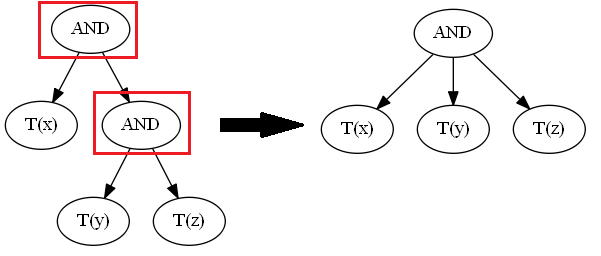
\includegraphics[scale=0.4]{Bilder/op_comp.png}
\caption{Operatorkompression}
\label{fig:opcomp}
\end{figure}

Gegeben sei der ZQL-Parsebaum $B=(V,E)$. Es sei $children(v) = \{ w : w\in V \wedge (v,w)\in E\}$, also die Menge aller Kindknoten von $v$. Gilt $v\in V$ und sei $v$ ein innerer Knoten, dann muss $v$ einen Operator repräsentieren, den wir mit $\mathit{operator}(v)$ erhalten. Gibt es einen Knoten $w\in children(v)$ mit $\mathit{operator}(v)=\mathit{operator}(w)$, so wird Knoten $w$ eliminiert und alle Kindknoten von $w$ werden zu Kindknoten von $v$, also $children(v) := children(v) \cup children(w) \setminus \{w\}$ und $E=E\backslash \{ (w,x) : x\in children(w)\} \cup \{(v,x) x\in children(w)\}$ und $V=V\backslash \{w\}$.

Im Sinne des Vergleiches der Komplexität der Musterlösung mit der Komplexität der Lösung des Lernenden ist es sinnvoll zu speichern, ob und wie oft eine solche Operatorkompression durchgeführt werden musste.

\subsubsection{NOT auflösen}

Im nächsten Schritt möchten wir auftretende \verb|NOT|-Operatoren entfernen. Dies geschieht, indem der Operator \verb|NOT| im Parserbaum nach unten geschoben wird. Dabei werden die \textit{DE MORGAN}-Regeln angewendet. 

\begin{tabular}{ll}
Eingabe: & Umwandlung Teil 1:\\
\verb|not ((a > 5)  and ((b > 5) or (c > 5)))| & \verb|(not(a > 5) or not((b > 5) or (c > 5)))|\\
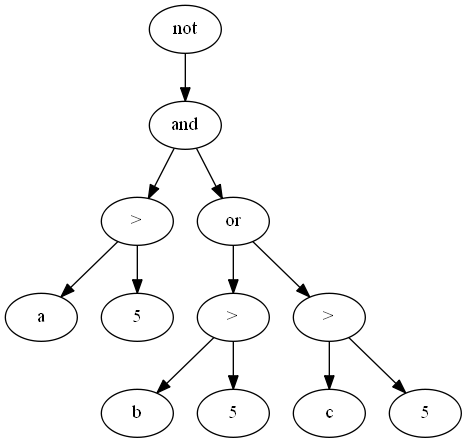
\includegraphics[scale=0.45]{Bilder/not_graph1.png} & 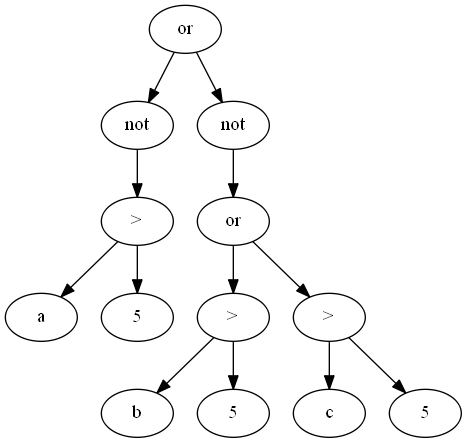
\includegraphics[scale=0.45]{Bilder/not_graph2.png}\\
\end{tabular}

\begin{tabular}{ll}
Umwandlung Teil 2: & Umwandlung Teil 3:\\
\verb|((a <= 5) or (not(b > 5) and not(c > 5)))| & \verb|((a <= 5) or ((b <= 5) and (c <= 5)))|\\
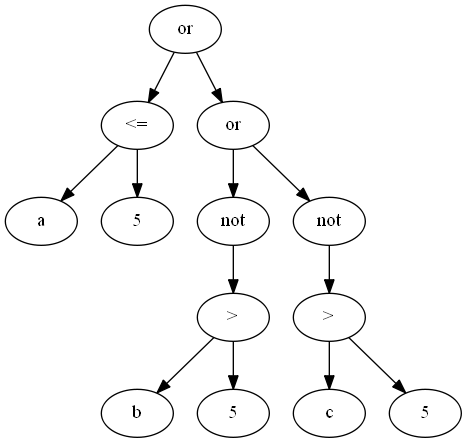
\includegraphics[scale=0.45]{Bilder/not_graph3.png} & 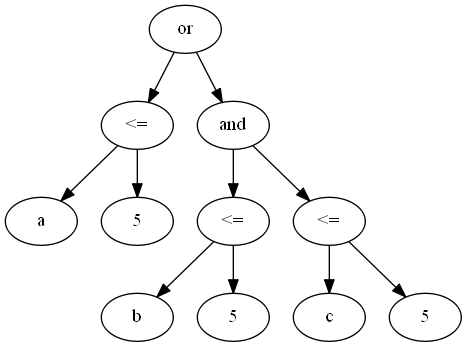
\includegraphics[scale=0.45]{Bilder/not_graph4.png}\\
\end{tabular}


\subsubsection{Anwenden des Distributivgesetzes}

Im letzten Schritt haben wir die Formel \verb|((a <= 5) or ((b <= 5) and (c <= 5)))| erhalten. Durch Anwenden des Distributivgesetzes können wir diese Formel im letzten Schritt umformen zu: \verb|((a <= 5) or (b <= 5)) and ((a <= 5) or (c <= 5))|.

Im Allgemeinen durchsuchen wir den Parserbaum auf Konstellationen, in denen ein Knoten mit dem Operator \verb|OR|, Elternknoten von einem \verb|AND|-Knoten ist. Dann müssen wir auf diesen Teilbaum das Distributivgesetz anwenden. Wir wiederholen diesen Vorgang, bis kein \verb|OR|-Knoten mehr Vorfahr eines \verb|AND|-Knotens ist.

\subsection{Ersetzung von syntaktischen Varianten}

Um eine Anfrage zu standardisieren müssen wir den syntaktischen Zucker entfernen. Dies geschieht, indem man nur eine syntaktische Schreibweise anerkennt und alle anderen Schreibweisen in die zulässige umgewandelt. 

Mit dem Operator \verb|BETWEEN| testen wir, ob ein gegebener Ausdruck zwischen zwei Werten, lower und upper, befindet. Wir schreiben den Ausdruck \verb|e BETWEEN lower AND upper| äquivalent um, indem wir nur Vergleichsoperatoren benutzten. \\Unser Ausdruck lautet dann: \verb|e >= lower AND e <= upper|.

Der Operator \verb|IN| prüft, ob ein gegebener Ausdruck einem bestimmten Wert aus einer Liste zugewiesen ist. Die Liste kann dabei als Unterabfrage oder als Liste von Konstanten beschrieben werden. Handelt es sich um eine Liste von Konstanten, so können wir \\\verb|e IN (const1, const2, ..., constn)| ersetzen indem wir prüfen, ob \verb|e| einen der konstanten Werte annimmt. Wir verknüpfen also $n$ Vergleiche disjunktiv miteinander. Wir erhalten dadurch: \verb|e = const1 OR e = const2 OR ... OR e = constn|.

Ähnlich dazu verhält sich der Operator \verb|ALL|. Er tritt in folgender Form auf:\\
\verb|operand comparison_operator ALL (subquery)|. Dabei kann \verb|subquery| auch eine Liste von Konstanten sein. Es wird in jedem Fall geprüft, ob der Operand und jedes der Listenelemente in der Vergleichsrelation enthalten ist. Haben wir als \verb|subquery| eine Liste von Konstanten, so ist dies äquivalent mit dem paarweisen Vergleich von \verb|operand| und jedem Listenelement. Diese $n$ Vergleiche werden dann konjunktiv verknüpft, also: \\
\verb|operand operator elem1 AND ... AND operand operator elemn|. 
Diese syntaktische Anpassung ist nicht im Programm enthalten, da der ZQL-Parser keine Listen unter \verb|ALL| versteht.

Der Operator \verb|ANY| ist beinahe äquivalent zu \verb|ALL| mit dem Unterschied, dass die entstandene Liste der Vergleiche nicht konjunktiv, sondern disjunktiv verknüpft wird.

Befindet sich im \verb|WHERE|-Teil eine \verb|EXISTS|-Unterabfrage, so können wir den \verb|SELECT|-Teil dieser Unterabfrage vereinfachen. Da wir nur wissen wollen, ob es Ergebnistupel aus der Unterabfrage gibt, benötigen wir keine konkreten Spalten aus der Unterabfrage. Daher ersetzen wir den \verb|SELECT|-Teil von \verb|EXISTS|-Unterabfragen zu: \verb|SELECT 1|. Ein Beispiel dieser Umwandlung ist in Abbildung \ref{fig:exists_ex1} zu sehen.

\begin{figure}[H]
\begin{verbatim}
SELECT e.sal FROM emp e WHERE EXISTS (
    SELECT expression FROM dept d 
    WHERE e.deptno = d.deptno )
    
SELECT e.sal FROM emp e WHERE EXISTS (
    SELECT 1 FROM dept d 
    WHERE e.deptno = d.deptno )
\end{verbatim}
\caption{Umwandlung des SELECT-Teils einer EXISTS-Unterabfrage}
\label{fig:exists_ex1}
\end{figure}


%\begin{figure}[H]
%\begin{tabular}{ccl}
%\verb|A BETWEEN B AND C| & $\to$  & \verb|A >= B AND A <= C|\\
%\verb|SELECT ALL| & $\to$ & \verb|SELECT|\\
%\verb|ORDER BY VAR ASC| &  $\to$ & \verb|ORDER BY VAR|\\
%\verb|A IN ('X', 'Y', 'Z')| & $\to$ & \verb|A = 'X' OR A = 'Y' OR A='Z'|\\
%\verb|EXISTS (SELECT A,B,C ...)| & $\to$ & \verb|EXISTS (SELECT 1 ...)|\\
%\end{tabular}
%\caption{Entfernen von syntaktischen Varianten}
%\end{figure}

\subsubsection*{Unteranfragen}

Es ist bekannt, dass sämtliche Typen von Unteranfragen eliminiert oder durch \verb|EXISTS|-Anfragen ersetzt werden können. Streng genommen handelt es sich hier zwar um mehr als nur eine syntaktische Variante, aber dennoch wollen wir das Ersetzen von Unteranfragen in diesem Abschnitt betrachten.

Wir behandeln hier nur echte Unterabfragen, das heißt die Unterabfrage darf keine Liste von Konstanten sein. Ist die Unterabfrage eine Liste, \mbox{z. B.} bei \verb|ALL, ANY| oder \verb|IN| gehen wir vor, wie im vorherigen Abschnitt beschrieben.

Für alle folgenden Umwandlungen müssen bestimmte Voraussetzungen erfüllt werden. Diese betrachten wir näher nachdem wir die Umformungen besprochen haben. Alle diese Umformungen sind auch in unserem Programm zu finden.

\subsubsection*{ALL-Unterabfragen}

\verb|ALL|-Unterabfragen haben immer das Muster:\\ \verb|operand comparison_operator ALL (subquery)|.\\ Dabei handelt es sich bei einem \verb|comparision_operator| um einen Operator aus der Menge: \verb|{=,<>,>,<,>=,<=}|. Die Unterabfrage \verb|subquery| liefert ein Attribut. Dann wird so verfahren, wie bereits im letzten Abschnitt erklärt wurde. Unser Ziel ist es, diese Unterabfrage, wenn möglich, zu ersetzen durch eine \verb|EXISTS|-Unterabfrage. Um diese Umwandlung nachzuvollziehen, wandeln wir zunächst die Unterabfrage mit \verb|ALL| in eine Unterabfrage mit \verb|ANY| um. Dazu ersetzen wir den \verb|comparison_operator| mit seinem gegenteiligem Operator. Folgende Paare sind jeweils voneinander gegenteilige Operatoren: \verb|{ {<,>=}, {>,<=}, {=,<>} }|. Danach ersetzen wir \verb|ALL| mit \verb|ANY| und kapseln die gesamte Unterabfrage mit einem \verb|NOT|. \newpage

%\begin{figure}
\begin{lstlisting}[mathescape]
WHERE $t_1$ comparison_operator ALL (
	SELECT $t_2$
	FROM $R_1$ $X_1$, ..., $R_n$ $X_n$
	WHERE ($\varphi$)
)

Geschrieben als ANY-Unterabfrage:
WHERE NOT( $t_1\ $opposite(comparison_operator$)$ ANY (
	SELECT $t_2$
	FROM $R_1$ $X_1$, ..., $R_n$ $X_n$
	WHERE ($\varphi$) ) 
)
\end{lstlisting}

Diese \verb|ANY|-Unterabfrage können wir nun in eine \verb|EXISTS|-Unterabfrage transformieren. Wie das genau durchgeführt wird, behandeln wir im nächsten Absatz.

%\caption{Umwandeln von \verb|ALL|- in \verb|ANY|-Unterabfrage}
%\label{fig:all_ex2}
%\end{figure}

\subsubsection*{ANY/ SOME-Unterabfragen}

Da \verb|SOME| und \verb|ANY| äquivalente und synonyme Schlüsselworte sind, ersetzen wir das Schlüsselwort \verb|SOME| durch \verb|ANY|. Damit reicht es im Folgenden nur \verb|ANY|-Unterabfragen zu betrachten. Eine solche Unterabfrage kann in eine \verb|EXISTS|-Unterabfrage umgewandelt werden. Dazu verknüpfen wir den Vergleichsoperator mitsamt linken Operanden konjunktiv mit dem \verb|WHERE|-Teil der Unterabfrage. Als rechten Operanden wählen wir das Attribut, welches sich im \verb|SELECT|-Teil der Unterabfrage befindet. Die Umwandlung findet also nach folgendem Muster statt:

\begin{lstlisting}[mathescape]
WHERE $t_1\ $comparison_operator ANY (
	SELECT $t_2$
	FROM $R_1$ $X_1$, ..., $R_n$ $X_n$
	WHERE ($\varphi$) 
) 

Geschrieben als EXISTS-Unterabfrage:
WHERE EXISTS( 
	SELECT 1
	FROM $R_1$ $X_1$, ..., $R_n$ $X_n$
	WHERE ($\varphi$ 
	AND $t_1$ comparison_operator $t_2$ )
)
\end{lstlisting}

\subsubsection*{IN-Unterabfragen}

Das Schlüsselwort \verb|IN| ist lediglich ein Synonym für \verb|= ANY|. Diese Unterabfragen sind daher ein Spezialfall der bereits betrachteten \verb|ANY|-Unterabfragen.

\subsubsection*{Voraussetzungen}

Alle, eben genannten, Umwandlungen können nur durchgeführt werden, wenn bestimmte Bedingungen erfüllt sind.

\begin{enumerate}
\item Alle Tupelvariablen, die in $t_1$ vorkommen, müssen sich unterscheiden von allen $X_i$. Erreicht wird dies ggf. durch Umbenennung der $X_i$, da diese nicht für die eigentliche (Ober-)anfrage wichtig sind.\\
\textbf{Unser Programm:} Wie bereits deutlich gemacht, erstellen wir unsere Tupelvariablen iterativ. In einer Unterabfrage wird die Iteration fortgeführt. Daher ist es nicht möglich, dass Tupelvariablen aus $t_1$ gleich sind mit einer $X_i$.
\item Wenn $t_1$ Attributreferenzen $A$ ohne Tupelvariable enthält, dann dürfen die $R_i$ kein Attribut $A$ haben. Erreicht wird dies, indem ggf. die Tupelvariable eingeführt wird.\\
\textbf{Unser Programm:} Wir erstellen für jede Attributreferenz eine Tupelvariable und erfüllen daher auch die Bedingung 2.
\item Die Unteranfrage für $t_2$ darf keine Nullwerte liefern, wenn die Unterabfrage negiert ist. \\
\textbf{Unser Programm:} Behandeln wir eine nicht-negierte Unterabfrage, können wir diesen Punkt ignorieren. Haben wir aber eine negierte Unterabfrage, dann prüfen wir, ob die Unterabfrage Spalten liefert, die nach Definition \verb|NULL| sein könnten. Ist dies der Fall, gehen wir vereinfacht davon aus und passen die Unterabfrage nicht an.
\end{enumerate}

\subsubsection{Andere Unteranfragen}

Ungewöhnlichere Unterabfragen, wie \mbox{z. B.} Unterabfragen unter \verb|FROM|, werden hier nicht betrachtet. Im Allgemeinen werden solche Unterabfragen kaum gebraucht und machen die Anfrage meist nur viel komplexer als notwendig. Der vorgestellte Parser unterstützt außerdem keine Unterabfragen unter \verb|FROM|. Er versteht nur Listen von Relationen mit Tupelvariablen.

\subsection{Operatorenvielfalt}

Im folgenden Abschnitt soll geklärt werden wie mit verschiedenen Schreibweisen von ein- und demselben Ausdruck umgegangen werden soll. Betrachtet man sich \mbox{z. B.} \verb|A > 5| ist dieser Ausdruck äquivalent mit \verb|5 < A|. Wenn wir wissen, dass \verb|A| ein ganzzahlige Variable ist, dann sind auch folgende Ausdrücke äquivalent: \verb|A >= 6| sowie \verb|6 <= A|. Wir betrachten nun zwei verschiedene Ansätze, die diese Probleme lösen sollen. Der erste Ansatz beschäftigt sich damit, alle implizierten Schreibweisen mit in die Formel aufzunehmen. Damit stellt man sicher, dass sich alle korrekten Schreibweisen einer Formel in der Anfrage befinden. Der zweite Ansatz beschäftigt sich damit, nur bestimmte Schreibweisen zuzulassen und alle anderen durch die zulässigen zu ersetzen.

\subsubsection{Analyse der unterschiedlichen Operatoren}

Wir unterscheiden im Wesentlichen zwei Arten von Operatoren. Zunächst haben wir Operatoren, bei denen wir die Operanden in beliebiger Reihenfolge anordnen können. Wir nennen diese Operatoren, kommutative Operatoren. Dies sind \verb|{ =, AND, OR, +, *}|. Alle anderen Operatoren sind demnach nicht-kommutativ, da wir die Reihenfolge der Operanden nicht ändern können, ohne den Ausdruck zu verfälschen. Zu dieser Gruppe von Operatoren zählen \verb|{ >=, >, <, <=, -, /, }|. Eine dritte Gruppe bilden unäre Operatoren, die nur einen Operanden kennen. Diese Gruppe ist aber im Sinne der Anordnung uninteressant, da wir hier keine mehrdeutig aufgeschrieben Varianten haben.

Ziel ist es nach wie vor, eine gewisse Ordnung zu definieren, so dass nach der Standardisierung semantisch gleiche Anfragen auch syntaktisch gleich sind. Betrachten wir nun einen Ausdruck mit einem Operator $op$ und $n$ Operanden, die wir fortlaufend mit $\mathit{child_1},...,\mathit{child_i},...,\mathit{child_n}$ bezeichnen. Ist $op$ ein kommutativer Operator, so können wir die Operanden $child_i$ beliebig anordnen, ohne den Sinn des Ausdrucks zu verändern. Dies tun wir, indem wir eine bestimmte Sortierreihenfolge etablieren. Diese finden wir im späteren Abschnitt \ref{subsec:sort}.

Hat eine Formel einen nicht-kommutativen Operator, so ist diese Sortierung nicht möglich. In einem solchen Fall müssen wir sicherstellen, dass sowohl die Musterlösung als auch die Lösung des Lernenden, die gleiche Repräsentation der Formel enthält. Ist \verb|a| eine Variable vom Typ \verb|INT|, dann sind verschiedene Repräsentationen von: \verb|a < 5| \mbox{z. B.} \verb|5 > a, a <= 4, 4 >= a|. Wir untersuchen nun zwei Ansätze, die sich mit diesem Problem beschäftigen. Im ersten Ansatz fügen wir, zu einer Formel mit einem nicht-kommutativen Operator, alle implizierten Schreibweisen hinzu. Ein Beispiel dafür ist in Abbildung \ref{fig:sampleadd} zu sehen. Im zweiten Ansatz analysieren wir die Formel mit dem nicht-kommutativen Operator und wählen eine bestimmte Repräsentation dieser Formel aus. Dadurch ist sichergestellt, dass sich in allen standardisierten SQL-Anfragen nur eine bestimmte Version der Formel befindet. Ein Beispiel dafür finden wir in Abbildung \ref{fig:samplerep}. Wir gehen davon aus, dass das Attribut \verb|sal| ganzzahlig ist.

\begin{figure}[H]
\centering
\begin{verbatim}
Eingabe: SELECT * FROM emp e WHERE e.sal >= 1001
Ausgabe: SELECT * FROM emp e 
         WHERE e.sal > 1000 AND 1000 < e.sal
         AND e.sal >= 1001 AND 1001 <= e.sal
\end{verbatim}
\caption{Beispiel für das Hinzufügen implizierter Formeln}
\label{fig:sampleadd}
\end{figure}

\begin{figure}[H]
\centering
\begin{verbatim}
Eingabe: SELECT * FROM emp e WHERE e.sal >= 1001
Ausgabe: SELECT * FROM emp e WHERE e.sal > 1000
\end{verbatim}
\caption{Beispiel für das Auswählen eines Repräsentanten}
\label{fig:samplerep}
\end{figure}

Haben wir weitere Formeln hinzugefügt, so müssen wir die konjunktive Normalform wiederherstellen, da wir nun \verb|AND|-Knoten hinzugefügt haben, die nicht auf der Wurzelebene sind. 

In unserem Programm verwenden wir den Ansatz: Hinzufügen von implizierten Formeln, der im Folgenden als erster Ansatz vorgestellt wird.

\subsubsection{Hinzufügen implizierter Formeln}
\label{subsubsec:implicitformulas}

Wie bereits im vorherigen Beispiel ersichtlich, sind die hinzugefügten Formeln redundant und tragen nicht effizient zur Beschleunigung der Anfrage bei. Es soll hier lediglich sichergestellt werden, dass alle möglichen äquivalenten Formeln auftreten, da wir nicht wissen, was der Lernende für einen Repräsentanten der Formeln wählen wird. Weiterhin muss bemerkt werden, dass dadurch die gesamte SQL-Anfrage enorm aufgebläht wird. Es ist daher unbedingt notwendig, die Originalanfrage zu speichern. Weiterhin muss das Programm eine Verbindung zwischen den Formeln der Originalanfrage und den Formeln der veränderten, aufgeblähten Anfrage herstellen. Dem Lernenden soll in einem Feedback nur Fehler in der Originalanfrage aufgezeigt werden. Da intern aber mit der aufgeblähten Anfrage gearbeitet wird, muss beim Auftreten eines Fehlers oder Hinweises nachgeschlagen werden, von welchem Teil der Originalanfrage der Teil entstammt, der jetzt den Fehler auslöst.

Im Folgenden listen wir Mengen $M_i$ von Ausdrücken auf. Finden wir in der zu bearbeitenden SQL-Anfrage eine Formel $f$, die auf einen Ausdruck $a\in M_i$ passt, dann verknüpfen wir alle Ausdrücke $\{b : b\in M_i \wedge b \neq a\}$ konjunktiv mit $f$. Dabei sind alle Variablennamen $A,B,C$ keine (komplexen) Ausdrücke. Es handelt sich also jeweils um Blattknoten im Parserbaum. Ferner bezeichnen wir $X,Y$ als numerische Konstanten. Wir setzen dabei voraus, dass eine Vorauswertung von arithmetischen Ausdrücken stattgefunden hat. Damit können wir auch sicher sein, dass in $M_2$ keine Division durch 0 stattfindet, da $A=0$ wenn $B=0$ oder $C=0$.\\

\begin{tabular}{ll}
$M_1$ & $\{\ A=B-C\ ,\ C=B-A\ ,\ B=A+C\ \}$\\
$M_2$ & $\{\ A=B\cdot C\ ,\ C=A / B\ ,\ B=A / C\ \}$\\
$M_3$ & $\{\ A>B-C\ ,\ C>B-A\ ,\ B<A+C\ \}$\\
$M_4$ & $\{\ A<B-C\ ,\ C<B-A\ ,\ B>A+C\ \}$\\
$M_5$ & $\{\ A>B, B<A \}$\\
$M_6$ & $\{\ A\geq B, B\leq A \}$\\
$M_7$ & $\{\ A>X, A\geq X+\mathit{adjust}(A) \}$\\
$M_8$ & $\{\ A<X, A\leq X-\mathit{adjust}(A) \}$\\

\end{tabular}

Beim Vergleich mit $>$ und $<$ ist es wichtig zu wissen, wie viele Nachkommastellen die numerischen Variablen $A$ und $B$ besitzen. Es sei $\mathit{places}(A)$ die Anzahl der Nachkommastellen der Zahl $A$. Dann bezeichnen wir mit $\mathit{adjust}(A) = 1 / (10^{\mathit{places}(A)})$ einen angepassten Wert, der sich nach der Anzahl der Nachkommastellen der Variable A richtet.

Betrachten wir als Beispiel ein Attribut \verb|salary|, welches als \verb|NUMERIC(4,2)| definiert ist. Wir wissen also, dass \verb|salary| zwei Nachkommastellen hat. Betrachten wir nun die Aussage\\ \verb|salary >= 5|.
Wir haben auf einer Seite eine Variable (\verb|salary|) und auf der anderen Seite eine numerische Konstante (\verb|5|). Dieses Muster passt also auf $M_7$ und auf $M_6$. In $M_7$ heißt es $A\geq X+\mathit{adjust}(A)$. Bezogen auf unser Beispiel ist \verb|A=salary| und \verb|x+adjust(salary)=5|. Wir berechnen also: 
$$\mathit{adjust}(\mathit{salary}) = 1 / (10^{2}) = 1/100 = 0,01$$
Wir erhalten \verb|x=4,99|, weil \verb|x+0,01=5|. Somit ergänzen wir unsere Ausgangsformel\\ \verb|salary >= 5| konjunktiv mit \verb|salary > 4,99|. Weiterhin muss jetzt wegen $M_6$, \verb|5 <= salary|, und wegen $M_5$, \verb|4,99 < salary|, hinzugefügt werden.

Finden wir Ausdrücke mit $>,<,\leq,\geq$, welche als Argumente Variablen oder Konstanten haben, so unterscheiden wir also grundsätzlich drei Fälle:

Fall 1 $(M_5,M_6)$: Beide Operanden sind Variablen. In diesem Fall ergänzen wir nur den jeweils symmetrischen Operator. Da beide Operanden Variablen sind, macht es weniger Sinn jeweils $\leq,\geq$ oder $<,>$ zu ersetzen, da normalerweise ein künstliches Hinzufügen eines Summanden auf einer Seite die Anfrage unnatürlich aussehen lässt. Es ist aber auch kein Problem diese Ersetzungen dennoch durchzuführen, wenn beide Operanden Variablen sind. Die Anfrage wird dann natürlich noch weiter künstlich aufgebläht.

Fall 2 $(M_7,M_8)$: Einer der beiden Operanden ist eine numerische Konstante und der andere ist eine Variable. In diesem Fall fügen wir alle implizierten Gleichungen hinzu, also insbesondere die Operatoren $\leq,\geq,<,>$. Zu beachten ist hier, dass nicht nur Gleichungen der Form $A>X$ dazu führen, dass alle Ausdrücke von $M_7$ hinzugefügt werden. Auch wenn eine Gleichung der Form $Var1\geq 5.2$ auftaucht, werden Ersetzungen durchgeführt. Diese Gleichung passt auf das Muster $A\geq X+\mathit{adjust}(A)$. Angenommen $Var1$ hat maximal eine Nachkommastelle, so würden dann folgende Gleichungen impliziert werden: $\{\ Var1>5.1\ ,\ 5.1<Var1\ ,\ 5.2 \leq Var1\ \}$.

Fall 3: Beide Operanden sind numerische Konstanten. In dem Fall wird die logische Aussage ausgewertet. Wir verfahren dann wie in einer aussagenlogischen Formel gemäß den Gesetzen: 
\begin{center}
\begin{tabular}{lclcllclcl}
$(1)\,true $ & $\wedge$ & $ f$ & $\equiv$ & $ f$ & $(2)\,true $ & $\vee$ & $ f$ & $\equiv$ & $true$\\
$(3)\,false $ & $\wedge$ & $ f$ & $\equiv$ & $false$ & $(4)\,false $ & $\vee$ & $ f$ & $\equiv$ & $f$\\
\end{tabular}
\end{center}

Wir können diese ersetzten Werte in SQL allerdings nicht verwenden, da im Standard keine Unterstützung für konstante Wahrheitswerte existiert. Dennoch ist ZQL in der Lage diese Werte zu akzeptieren. Wir können damit eine BOTTOM-UP-Auswertung von konstanten Ausdrücken realisieren. Kommt dabei heraus, dass der komplette \verb|WHERE|-Teil aus \verb|false| besteht, so muss dem Nutzer eine Meldung angezeigt werden, dass seine SQL-Anfrage stets die leere Menge liefert.

In einem anschließenden Schritt werden arithmetisch/ logische Ausdrücke ausgewertet und durch ihre Ergebnisse ersetzt. Dieser Schritt muss BOTTOM-UP geschehen, damit man auch mehrere Ersetzungen nach oben, im Parserbaum, weiterreicht. Haben wir am Ende einen SQL-Ausdruck dessen \verb|WHERE|-Teil aus \verb|false| besteht, dann haben wir eine Anfrage gefunden, die immer das leere Ergebnis liefern wird. In diesem Fall müssen wir natürlich eine Fehlermeldung ausgeben.

Sollten wir durch das Hinzufügen implizierter Formeln jetzt einige Formeln doppelt in unserer Anfrage haben, so werden diese bei der Sortierung entfernt.

\subsubsection{Beschränkung der Operatorenvielfalt}

Ein weiterer Ansatz das Problem der äquivalenten Formeln zu Lösen, ist es bestimmte Operatoren zu >>verbieten<<. Das soll bedeuten, dass wir verbotene Operatoren definieren, welche am Ende der Umwandlungen nicht mehr in der SQL-Anfrage vorkommen dürfen. Dies wird erreicht, indem wir jeden verbotenen Operator umwandeln in einen zugehörigen, nicht-verbotenen Operator. Das Prinzip ähnelt dem eben Vorgestellten. Wir betrachten wieder die Mengen $M_i$. Des Weiteren hat jede Menge $M_i$ einen Repräsentanten $r(M_i)$. Finden wir nun in der zu bearbeitenden Anfrage eine Formel $f$, die auf eine der Ausdrücke $a\in M_i$ passt, so ersetzen wir $f$ mit $r(M_i)$.\\

Im Folgenden sind alle Variablennamen $A,B,C$ keine (komplexen) Ausrücke. Es handelt sich also jeweils um Blattknoten im Parserbaum. Ferner bezeichnen wir $X,Y$ als numerische Konstanten. Wir setzen dabei voraus, dass eine Vorauswertung von arithmetischen Ausdrücken stattgefunden hat. Damit können wir auch sicher sein, dass in $M_2$ keine Division durch 0 stattfindet, da $A=0$ wenn $B=0$ oder $C=0$. Folgende Tabelle soll die Mengen und deren Repräsentanten beschreiben:

\begin{tabular}{lll}
$i$ & $M_i$ & $r(M_i)$ \\
$1$ & $\{\ A=B-C\ ,\ C=B-A\ ,\ B=A+C\ \}$ & $B=A+C$\\
$2$ & $\{\ A=B\cdot C\ ,\ C=A / B\ ,\ B=A / C\ \}$ & $A=B\cdot C$\\
$4$ & $\{\ A>B-C\ ,\ C>B-A\ ,\ B<A+C\ \}$ & $A>B-C$ \\
$5$ & $\{\ A<B-C\ ,\ C<B-A\ ,\ B>A+C\ \}$ & $A<B-C$\\
$6$ & $\{\ A>B, B<A \}$ & $A>B$\\
$7$ & $\{\ A\geq B, B\leq A \}$ & $A\geq B$\\
$8$ & $\{\ A>X\ ,\ X<A,A\geq X+\mathit{adjust}(X)\ ,\ X\leq A - \mathit{adjust}(X)\ \}$ & $A>X$\\
\end{tabular}

Ein Beispiel soll das Vorgehen verdeutlichen.\\
Es sei unsere Ausgangsanfrage: \begin{verbatim}SELECT * FROM testtable WHERE X = 6 - Y\end{verbatim}

Die Formel $X=6-Y$ finden wir in $M_1$ in Form von $A=B-C$. Wir ersetzen nun also $X=6-Y$ mit dem Repräsentanten von $M_1$, und bekommen: \begin{verbatim}SELECT * FROM testtable WHERE 6 = X + Y\end{verbatim}

Ein Problem bei der Verwendung von Repräsentanten durch Einschränkung der Operatorenvielfalt ist, dass es zu überlappenden Mengen kommen kann. Damit ist gemeint, dass ein Ausdruck auf mindestens zwei Mengen $M_i$ und $M_j$ mit $i\neq j$ passt. In einem solchen Fall müssen die Mengen $M_i$ und $M_j$ genauestens untersucht werden. Im Normalfall ist dann eine Verschmelzung von $M_i$ und $M_j$ möglich, da diese Äquivalenzklassen beschreiben und ein Element in nur genau einer Äquivalenzklasse vorhanden sein kann.

\subsubsection{Einschränkungen bei arithmetischen Ausdrücken}
\label{subsubsec:arithmetic}

Bevor wir zur Diskussion beider Ansätze kommen, müssen wir noch erklären, was die beiden Ansätze bisher nicht leisten können. Für beide Ansätze haben wir angenommen, dass arithmetische Ausdrücke maximal aus zwei Operanden auf der komplexen Seite bestehen. Natürlich können in der Praxis auch komplexere Ausdrücke auftauchen. Diese Arbeit aber entsteht im Rahmen einer Lernplattform. In der Lehre kommt es selten vor, dass arithmetische Ausdrücke im Übermaß benutzt werden. Wenn sie auftauchen, sind sie auch meistens auf zwei Operanden beschränkt. Es ist kaum von Nöten, komplexe arithmetische Ausdrücke in der SQL-Anfrage zu verwenden. Im Rahmen dieser Arbeit betrachten wir solche Ausdrücke also immer mit maximal zwei Operanden auf der komplexeren Seite. Dies begründet sich auch in der zunehmenden Schwierigkeit solche komplexen Ausdrücke zu behandeln, wie wir im Folgenden sehen werden.

Wir wollen uns dennoch mit der Frage beschäftigen: Wie könnte man komplexere arithmetische Ausdrücke anpassen? Die folgenden Ansätze sind theoretische Überlegungen und stellen kein vollendetes Konzept dar. Wir gehen in unserem Programm trotz der folgenden Diskussion von der Beschränktheit der arithmetischen Ausdrücke aus.

\subsubsection{Komplexere arithmetische Ausdrücke -- Standardisierung}

Zunächst betrachten wir den Standardisierungsansatz. Hier möchten wir alle implizierten Gleichungen hinzufügen, sodass wir sicher gehen können, dass alle möglichen äquivalenten Gleichungen auftauchen. Dies gestaltet sich für komplexere arithmetische Ausdrücke schwierig. Es müssen alle Gleichungen, die durch äquivalente Umformungen entstehen können, errechnet werden, um sie dann der Lösung hinzuzufügen. Letztendlich führt uns diese Problematik zur Permutation aller Operanden. Für einen solchen Ansatz müssten alle Operatoren kommutativ sein. Wir behelfen uns in diesem Fall, indem wir die Operatoren $-$ und $/$ umschreiben in $+$ und $*$. Es folgt ein Beispiel:

\begin{tabular}{lll}
$A=B+C-D-E+F$ & $\to$ & $A=B+C+(-D)+(-E)+F$\\
$A=B*C/D/E*F$ & $\to$ & $A=B*C*(1/D)*(1/E)*F$\\
\end{tabular}

Nun können wir die Reihenfolge der Operanden permutieren. Im letzten Schritt müssen wir auch jeden Operanden auf jede Seite der Gleichung bringen und wieder die Reihenfolge der Operanden permutieren. So erhalten wir alle möglichen Schreibweisen eines komplexen arithmetischen Ausdrucks. Zu beachten ist, dass auf diese Weise schnell, sehr viele Gleichungen produziert werden. Dies macht die Lösung stark unübersichtlich. Zu bemerken ist weiterhin, dass gemischte Ausdrücke bezüglich $+$ und $*$ deutlich schwerer zu behandeln sind, als solche, die nur $+$ oder $*$ enthalten.

\subsubsection{Komplexere arithmetische Ausdrücke -- Operatorenbeschränkung}

Im zweiten Ansatz gestaltet sich das Problem etwas einfacherer. Wie bereits im ersten Ansatz eliminieren wir die Operatoren $-$ und $/$. Da wir am Ende nur eine Schreibweise als zugelassen betrachten, müssen wir nun festlegen, welche Schritte an jedem Ausdruck ausgeführt werden müssen. Wir entscheiden uns für folgende Konvention: Alle Variablen werden via äquivalenten Umformungen auf die linke Seite der Gleichung gebracht und alle numerischen Konstanten werden auf die rechte Seite der Gleichung gebracht. Im nächsten Schritt entfernen wir doppelte Minus- bzw. Divisionszeichen, aus $-(-2)$ wird also $+2$ und aus $1/1/E$ wird $E$. Nun rechnen wir den Wert des arithmetischen Ausdrucks auf der rechten Seite aus, da dieser nun nur noch aus Konstanten besteht. Die Linke Seite sortieren wir lexikographisch nach Namen der Variablen. Es muss daran erinnert werden, dass diese Namen automatisch generiert worden sind, sodass sichergestellt ist, dass wir Übereinstimmungen später finden können.

Zusammenfassend kann gesagt werden, dass eine Behandlung von komplexeren arithmetischen Ausdrücken möglich, aber nicht einfach umzusetzen ist. Wir haben nur Ansätze präsentiert, die in einem ausgearbeiteten Zustand das Problem der Standardisierung solcher arithmetischen Ausdrücke lösen könnten. Denkbar wären auch andere Ansätze, wie \mbox{z. B.} mehrfaches substituieren von zwei Operanden zu einer Variablen.  Alles in allem bedarf es bei diesem Problem noch weiterer Forschung.

%genaueres Vorgehen unklar

\subsubsection{transitiv-implizierte Formeln}

Formeln können auch transitiv-impliziert sein. Steht in der Musterlösung die Formel \verb|A>B AND B>C| und der Student hat geschrieben \verb|A>B AND A>C AND B>C|, so sind beide Aussagen logisch identisch. Leider erkennt dies unser bisheriger Ansatz nicht. Um solche Formeln zu erkennen, müssen wir auch alle transitiv-implizierten Formeln hinzufügen. Dabei gibt es verschiedene Fälle: 

Existiert in der Formel nur eine Relation $R$, so wie im Beispiel eben $R=\ '>'$, dann können wir im Ansatz des Hinzufügens implizierter Formeln die transitive Hülle von $R$ berechnen und die entstandenen Paare der Ausgangsformel hinzufügen. Wollen wir keine implizierten Formeln hinzufügen, sondern nur bestimmte Schreibweisen erlauben, so können wir zunächst die transitive Hülle $R^+$ berechnen und danach eine transitive Reduktion durchführen. Zu beachten ist bei diesem Ansatz, dass es nicht für jede Relation eine eindeutige transitive Reduktion gibt. 

Komplexer wird das Problem, wenn eine Formel verschiedene Relationen enthält, wie \mbox{z. B.} \\\verb|A>B AND B=9|. Diese Formel impliziert eine weitere Formel transitiv, weil die Relationen $>$ und $=$ zueinander kompatibel sind. Inkompatible Relationen sind jeweils $>,\geq$ zu $\leq,<$. Die Relation $=$ ist zu jedweder Relation kompatibel. Haben wir also eine Mischformel mit mehreren kompatiblen Relationen, dann ordnen wir das entstehende transitive Paar der allgemeineren Relation zu. In unserem Beispiel entsteht das Paar $(A,9)$. Da $>$ allgemeiner ist als $=$, ordnen wir $(A,9)$ der Relation $>$ zu. Auch hier können wir die implizierten Formeln der Ausgangsformel hinzufügen (Ansatz Hinzufügen der Implikationen) oder danach die transitive Reduktion berechnen, wie oben bereits erwähnt wurde. Ein Ansatz eines Algorithmus für solche Mischformeln wäre einen Graph zu erzeugen mit Operanden als Knoten und Relation als Kantenbeschriftung. Zwei Knoten sind genau dann miteinander verbunden, wenn sie durch eine Relation $R_i$ miteinander in der Formel verknüpft sind. $R_i$ ist dann auch die Kantenbeschriftung. Wenn auf einem Pfad alle Relationen zueinander kompatibel sind, wird mit üblichen Methoden die transitive Hülle bestimmt, indem neue Kanten eingezeichnet werden. Beschriftet werden diese Kanten mit dem allgemeinsten Vertreter der Relationen, die auf dem Pfad liegen. So erhalten wir alle transitiv-implizierten Paare.

\subsubsection{Implizierte Domänen}

Ein weiterer Problempunkt sind implizierte Domänen von Attributen. Es geht darum zu erfassen, welchen Wertebereich einzelne Attribute durch die Formeln in der SQL-Anfrage zugewiesen bekommen. Dabei können semantische Widersprüche entdeckt werden, wie \mbox{z. B.} \verb|A>9 AND A<9|. Diese Widersprüche führen meist zu einer leeren Antwort des SQL-Systems. Eine Hinweis würde dem Lernenden klar machen, dass diese Bedingung wahrscheinlich nicht gewollt ist. Die Erfassung des Wertebereichs deckt aber auch weitere Einsatzgebiete ab. So können auch unnötige Bedingungen erkannt werden, wie \mbox{z. B.} \verb|A>9 AND A>5|. Die letzte Bedingung wird ja bereits durch die erste Bedingung impliziert. Unser Matching-Ansatz würde in diesem Fall die Lösungen nicht unifizieren können, obwohl sie äquivalent sind. Man könnte hier aber auch argumentieren, dass die Lösung des Lernenden unnötige Formeln enthält, die keinen Nutzen für die Anfrage haben, und damit unser System, korrekterweise, keine Übereinstimmung erkennt. Andererseits wäre es hilfreich, wenn ein vorgeschalteter Semantikprüfer solche Probleme erkennt, um entweder den Lernenden vorab ein Feedback zu geben oder, um solche unnötigen Formeln bei der Bearbeitung zu ignorieren. 

Da dieses Problem eher in den Bereich Semantikprüfer gehört wird dieses Feature nicht im Programm auftauchen. Will man dem Programm später aber semantische Prüfer vorschalten, wäre dies auf jeden Fall ein wichtiges und sinnvolles Feature.

\subsubsection{Diskussion der beiden Ansätze}

Ein wesentlicher Punkt beim Vergleich beider Ansätze ist der Aufwand bzw. die Laufzeit. 

Betrachten wir zunächst den Ansatz des Hinzufügens von implizierten Formeln. Wir bezeichnen mit $length = \sum_{i=0}^n \vert M_i\vert$ die Gesamtanzahl aller Formeln über allen Mengen. Wir müssen in einer Tiefensuche jede Formel betrachten und mit allen Mengen $M_i$ mit $i\in \{1,2,...,n\}$ abarbeiten. Finden wir in einer Menge ein Muster wieder, so wird unsere Formel künstlich aufgebläht. Wir haben also für das Suchen eine maximale Laufzeit von $\mathcal{O}(\mathit{\vert Formeln\vert \cdot length})$. Das Einfügen der Formeln geschieht in konstanter Zeit $\mathcal{O}(k)$ mit $k= \max_{i\in [1,n]\cap \mathbb{N}} \vert M_i\vert$.

Beim anderen Ansatz werden bestimmte Operatoren verboten. Wir realisieren dieses Verbot wieder über eine Suche. Es muss auch hier jede Formel auf ein Muster in $M_i$ untersucht werden. Wir benötigen für das Suchen in diesem Ansatz also genau so viel Zeit, wie im ersten Ansatz. Auch das Ersetzen der Formeln hat keine Zeitersparnis gegenüber einem Hinzufügen von weiteren Formeln. Es muss bemerkt werden, dass in diesem Fall die Originalformel nicht weiter aufgebläht wird.

Da sich die Laufzeiten der beiden Varianten nicht unterscheiden, müssen andere Kriterien zum Vergleich herangezogen werden. Wichtig für eine Software ist nicht ausschließlich die Laufzeit, sondern auch die Wartbarkeit. Besonders bei Projekten, die im Rahmen einer Masterarbeit entstehen, ist es wahrscheinlich, dass der Autor sich später nicht mehr um das Projekt kümmern kann. Daher sollte man sich bei den hier vorliegenden Ansätzen fragen, welcher leichter wartbar und erweiterbar ist.

Muss das Programm erweitert werden und wir möchten den Ansatz des Hinzufügens implizierter Gleichungen verwenden, so muss lediglich eine weitere Menge $M_k$ erstellt werden. Der Algorithmus sucht dann auch automatisch nach Mustern in dieser neuen Menge und würde alle anderen Elemente dieser Menge konjunktiv-verknüpft zur Formel hinzufügen. 

Bei der Verwendung von eingeschränkten Operatoren gestaltet sich dieser Ansatz als schwierig. Hier muss man nicht nur die neue Menge $M_k$ angeben, sondern sich auch Gedanken machen, was ein geeigneter Repräsentant dieser Menge ist. Unter Umständen kann das Auswählen eines ungünstigen Repräsentanten zu unerwarteten Problemen, wie dem Verkomplizieren der Anfrage, führen.

Aufgrund dieser Umstände werden in unserer Anwendung implizierte Formeln hinzugefügt.

\subsection{Sortierung}
\label{subsec:sort}

Ein wesentlicher Aspekt bei der Standardisierung ist die Art der Sortierung. Dabei geht es im Folgenden um die Sortierung von atomaren Formeln und von zusammengesetzten Formeln. Wir betrachten dazu im Folgenden ZQL-Parserbäume. Im Wesentlichen sind dies gerichtete Bäume. Dabei stellen Knoten entweder Operatoren, Konstanten oder Variablen dar. Ein Operator $o_1$ kann natürlicherweise, als Kindknoten, wiederum einen Operator $o_2$ haben. Es sei $T(r)$ der Baum mit Wurzelknoten $r$. Wir bezeichnen mit $\mathit{children}(r)$, die Kindknoten von $r$ in folgender Art und Weise: $\textit{children}(r) = (c_1, c_2, ..., c_n)$. Dabei erscheint das Kind $c_i$ direkt links vom Kind $c_j$ genau dann, wenn $j = i + 1$. Anders ausgedrückt: Bei einer Breitensuche über $T(r)$ würden wir erst $c_i$ und im Anschluss daran $c_j$ auffinden, genau dann wenn $j = i + 1$.

Es sei $T(r)$ unser ZQL-Parserbaum. Ist der Operator, mit dem $r$ markiert ist, kommutativ, so können wir alle Kinder $c_i$ in beliebiger Reihenfolge permutieren und würden den Ausdruck, den $T(r)$ darstellt, nicht semantisch verändern. Für unsere Standardisierung ist es aber wichtig, dass wir dennoch eine Ordnung auf solchen Operatoren festlegen, damit unsere Parserbäume am Ende vergleichbar sind. Wir verwenden die Ordnung, die in Abbildung \ref{fig:sortorder} dargestellt ist. Ein niedrigerer Wert der $\mathit{order}$-Funktion bedeutet dabei eine höhere Priorität. Hat ein Kindknoten $c_i$ eine höhere Priorität als ein Kindknoten $c_j$, so steht $c_i$ weiter links in der Liste der Kinder. Zu beachten ist, dass Spaltennamen die höchste Priorität haben, gefolgt von den Konstanten, welchen die zweithöchste Priorität zugeordnet sind. Wir gehen bei der Herstellung der Ordnung im Baum von unten nach oben vor, also bottom-up. Damit können wir sicherstellen, dass beim Behandeln eines Knotens $v$, die Kinder $children(v)$ bereits korrekt sortiert sind, da wir ja mit den Blattknoten beginnen.

\begin{figure}[H]\
\begin{tabular}{|l|l|l|l|l|l|l|l|l|l|l|l|l|l|l|l|}
\hline
$r\in \textit{Relation}$ & Variable & Konstante & OR & $\le$ & $\ge$ & $<$ & $>$ & $=$& $+$ & $-$  & IS NULL\\\hline
$\textit{order}(r)$ & 1 & 2 & 3 & 4 & 5 & 6 & 7 & 8 & 9 & 10 & 11\\ 
\hline
\end{tabular}\newline
\begin{tabular}{|l|l|l|l|l|l|l|l|l|l|l|l|l|l|l|l|}
\hline
$r\in \textit{Relation}$ & IS NOT NULL & EXISTS & ANY & ALL  \\\hline
$\textit{order}(r)$ & 12 & 13 & 14 & 15 \\ 
\hline
\end{tabular}
\caption{Reihenfolge der Sortierung eines WHERE-Ausdrucks}
\label{fig:sortorder}
\end{figure}

Die Kinder vom Baum $T(r)$ müssen so angeordnet werden, dass für alle Kinder paarweise das Folgende gilt. Dabei seien $c_i,c_j\in\mathit{children}(r)$ und $r$ muss kommutativ sein.

$$\forall c_i,c_j : i\neq j \wedge order(c_i) \neq order(c_j) \to  ( i<j \leftrightarrow order(c_i) < order(c_j) ) $$

In Worten ausgedrückt: Für alle, paarweise verschiedenen, Kinder von $T(r)$ gilt: $c_i$ erscheint genau dann vor $c_j$ im Baum (bezüglich einer Breitensuche), wenn die oben angegebene Ordnung eingehalten wird. Dies wird initial nicht der Fall sein, daher müssen wir die Kinder so umsortieren, dass diese Bedingung erfüllt ist. 

Das klärt die Ordnung in unserem Parserbaum, wenn die Liste der Kinder stets mit paarweise unterschiedlichen Operatoren markiert ist. Es ist also ungeklärt wie wir Kindknoten sortieren, wenn diese mit gleichen Operatoren markiert sind. Dabei müssen wir zwei Fälle unterscheiden: Zwei Kindknoten markieren den gleichen Operator $o$ und zwei Kindknoten bezeichnen je Spaltennamen oder Konstanten. Beide Fälle lassen sich mit einer Methode lösen, die wir jetzt besprechen werden.

Markieren zwei Kindknoten $c_i,c_j$ den gleichen Operator $o = operator(c_i) = operator(c_j)$ so wissen wir, durch das BOTTOM-UP-Vorgehen bereits, dass die Kinder von $c_i$ und $c_j$ bereits korrekt sortiert sind. Wir untersuchen dann die beiden Bäume $T(c_i)$ und $T(c_j)$ rekursiv in einer Tiefensuche. Diese Tiefensuche geschieht in beiden Bäumen schrittweise und gleichzeitig. Wir bezeichnen die Knoten, bei denen sich die Tiefensuche gerade befindet als $v_i$ für den Baum $T(c_i)$ und $v_j$ für den Baum $T(c_j)$. Stellen wir in einem Schritt der Tiefensuche fest, dass die beiden Knoten sich unterscheiden, also $v_i \neq v_j$ gilt, so entscheiden wir anhand von $order(v_i)$ und $order(v_j)$ welcher Baum vor dem anderen erscheint. Hier gilt wieder, dass $T(c_i)$ vor dem Baum $T(c_j)$ erscheint, wenn $order(v_i) < order(v_j)$. 

Dieses Vorgehen funktioniert ebenso, wenn zwei Knoten entweder Spaltennamen oder Konstanten bezeichnen. Wir müssen hier nur festlegen, welcher Spaltenname bzw. Konstantenname Vorrang vor einem jeweils anderen hat. Wir entscheiden uns  für die lexikographische Ordnung. Haben wir bei der Tiefensuche nie den Fall, dass sich $v_i$ und $v_j$ unterscheiden, so sind beide Teilbäume identisch und die Reihenfolge ist nicht wichtig. Einer der Teilbäume wird im Anschluss der Sortierung dann entfernt, sofern der Elternknoten beider Teilbäume den Operator \verb|AND| oder \verb|OR| markiert.

Um den Prozess der Sortierung deutlich zu machen, betrachten wir zunächst das Verfahren als Pseudocode. Im Anschluss daran untersuchen wir ein detailliertes Beispiel. Zur Vereinfachung wird im Pseudocode Bubblesort zur Sortierung der Kinderelemente verwendet. In unserem Programm wird die Sortierung über die javaeigene Sort-Funktion geregelt, die mit Hilfe eines Comparers die Liste mit Quicksort sortiert. Weiterhin bezeichnen wir mit $a <_{lexik} b$, ob a lexikographisch kleiner ist als b. $swap(l_i,l_j)$ tauscht Element $l_i$ mit $l_j$ in der Liste $l=(l_1,...,l_n)$. 

Die Funktion \verb|dualDFS(v,w)| ist nicht im Pseudocode erläutert und wird daher kurz erklärt. Sie führt die schrittweise Tiefensuche auf $T(v)$ und $T(w)$ aus, wie oben beschrieben. Findet die Funktion zwei unterschiedliche Knoten $v_i$ und $v_j$ so gibt sie diese zurück. Andernfalls wird \verb|false| zurückgegeben.

Die Abbildungen \ref{fig:pesudocode1} und \ref{fig:pesudocode2} stellen den bisherigen Prozess dar.

\begin{figure}[H]
\lstset{tabsize=2,language=java,keywordstyle=\color{javapurple}\bfseries,
stringstyle=\color{javared},
commentstyle=\color{javagreen},
morecomment=[s][\color{javadocblue}]{/**}{*/}}

\begin{lstlisting}[mathescape]
sortiere_liste(Liste l=($l_1$,...,$l_n$)) {
	for(i=0; i<n; i++) {
		for(j=0; j<n; j++) {
			if ($l_i$ ist Konstante AND $l_j$ ist Konstante && $l_j <_{lexik} l_i$)
					swap($l_i,l_j$);
			else if ($l_i$ ist Spaltenname && $l_j$ ist Spaltenname
				&& $l_j <_{lexik} l_i$)
					swap($l_i,l_j$);
			else if ($l_i$ ist Operator AND $l_j$ ist Operator
				&& operator($l_j$) == operator($l_i$)) {
					$v_i, v_j$ = dualDFS($l_i,l_j$);
					if($v_i$ != false) {
						/*Sind $v_i,v_j$ Operatoren  entscheidet order(), 
						  ob getauscht wird. Sind beides Spaltennamen oder 
						  Konstanten entscheidet die lexikographische Ordnung 
						  */
						  maybe swap($v_i,v_j$);
					}
			} 
			else {
				  if(order($l_j$) < order($l_i$)) 
				  		swap($l_i,l_j$);
			}
		}
	}
}\end{lstlisting}			
\caption{Pseudocode: Sortieren von Listenelementen}
\label{fig:pesudocode1}
\end{figure}

\begin{figure}[H]
\lstset{tabsize=2,language=java,keywordstyle=\color{javapurple}\bfseries,
stringstyle=\color{javared},
commentstyle=\color{javagreen},
morecomment=[s][\color{javadocblue}]{/**}{*/}}
\begin{lstlisting}[mathescape]
sortiere(rootnode r) {
   if( children(r).isEmpty() )  return;        
   foreach( c in children(r)) {
      sortiere(c);
   }           
   if( kommutativ(r) ) {
      sortiere_liste(children(r));
   }
}
\end{lstlisting}
\caption{Pseudocode: Rekursiver Sortierprozess}
\label{fig:pesudocode2}
\end{figure}

Wir wollen dieses Verfahren nun an einem Beispiel verdeutlichen. Wir betrachten dazu den Ausdruck \verb| a>5 AND (2=b OR c IS NULL) AND (d=5 OR a<6)|, der in Abbildung \ref{fig:sort_1} als Baum dargestellt ist. Wir gehen davon aus, dass a,b,c und d Spaltennamen sind und keine Stringkonstanten.

\begin{figure}[H]
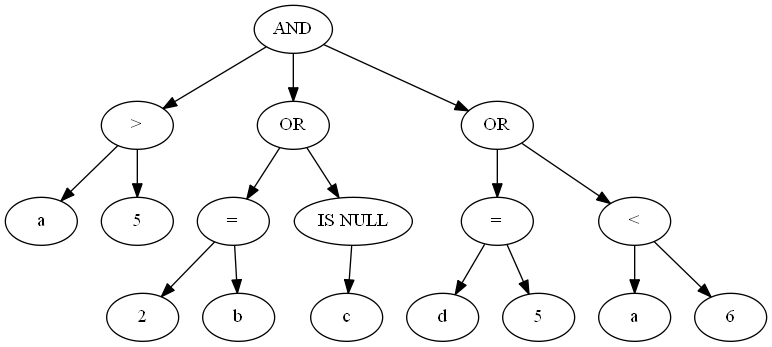
\includegraphics[scale=0.6]{Bilder/sort_1.png}
\caption{Sortierbeispiel: Ausgangsbaum}
\label{fig:sort_1}
\end{figure}

Wir führen zunächst den rekursiven Abstieg bis zu den Blattknoten durch. Wir steigen dann rekursiv auf und betrachten dabei jeweils Knoten, die Kindknoten besitzen. Als erstes Treffen wir dabei auf den Teilbaum, der den Ausdruck \verb|a > 5| repräsentiert. Da der Operator \verb|>| nicht-kommutativ ist, können wir die Reihenfolge der Kinder nicht ändern und fahren weiter fort. Im rekursiven Aufstieg treffen wir jetzt auf den Teilbaum, der den Ausdruck \verb|2=b| repräsentiert. Da \verb|=| kommutativ ist, sortieren wir nun die Kinder Anhand ihrer \verb|order()|-Werte. Dabei stellt sich heraus, dass \verb|order(b) = 1 < 2 = order(2)| und damit müssen die Kinder getauscht werden. Wir erhalten den Ausdruck: \verb|b=2|. 
Wir erreichen nun den Teilbaum, der den Ausdruck \verb|(b=2) OR (c IS NULL)| repräsentiert. Da aber \verb|order(=) < order(IS NULL)| ist, müssen wir die Kindknoten nicht vertauschen.
Wir fahren mit dem rekursiven Aufstieg fort und stoßen auf den Teilbaum, der \verb|d=5| repräsentiert. Da \verb|order(d) > order(5)| müssen wir die Kindknoten nicht tauschen. Wir fahren fort und treffen auf den Ausdruck \verb|a < 6| der ebenfalls nicht abgeändert werden kann, da \verb|<| nicht-kommutativ ist. 
Beim Aufstieg stoßen wir nun auf den Ausdruck \verb|(d=5) OR (a<6)|. Hier müssen wir eine Vertauschung der Kindknoten durchführen, da \verb|order(=) > order(<)|. Wie in Abbildung \ref{fig:sort_step1} zu erkennen ist, erhalten wir den Ausdruck \verb|(a<6) OR (d=5)|.

\begin{figure}[H]
\centering
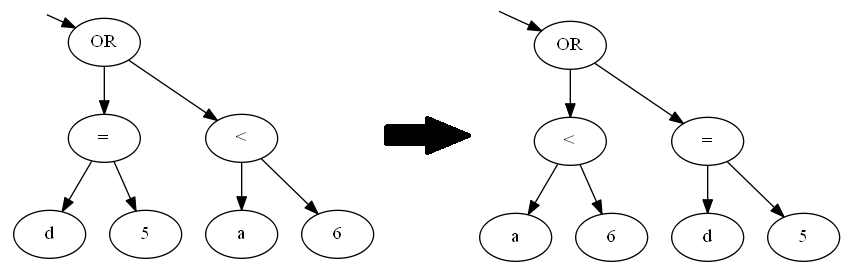
\includegraphics[scale=0.5]{Bilder/sort_step1.png}
\caption{Sortierbeispiel: Umsortierung der Teilbäume}
\label{fig:sort_step1}
\end{figure}

Nun treffen wir auf die zweite Ebene des Baumes und die Teilbäume mit den Wurzeln \verb|>, OR| und \verb|OR|. Da \verb|order(OR) < order(>)| gilt, ist klar, dass der Teilbaum mit \verb|>| als Wurzelknoten nach ganz rechts rücken muss. Noch zu klären ist, welcher der beiden Teilbäume mit \verb|OR| als Wurzel, als erstes Kind von \verb|AND| erscheint. Dazu müssen wir die schrittweise Tiefensuche auf beiden Bäumen ausführen. Wie wir in Abbildung \ref{fig:sort_step2} feststellen können, unterscheiden sich die Knoten bereits in der ersten Iteration der Tiefensuche.

\begin{figure}[H]
\centering
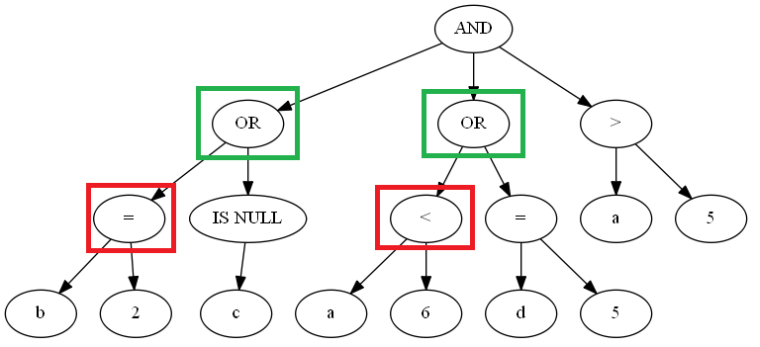
\includegraphics[scale=0.55]{Bilder/sort_step2.png}
\caption{Sortierbeispiel: Schrittweise Tiefensuche}
\label{fig:sort_step2}
\end{figure}

 Da \verb|order(<) < order(=)| müssen wir die Teilbäume mit \verb|OR| als Wurzel ebenso tauschen. Wir erhalten dann den Baum, der in Abbildung \ref{fig:sort_zwischen4} zu sehen ist.

\begin{figure}[H]
\centering
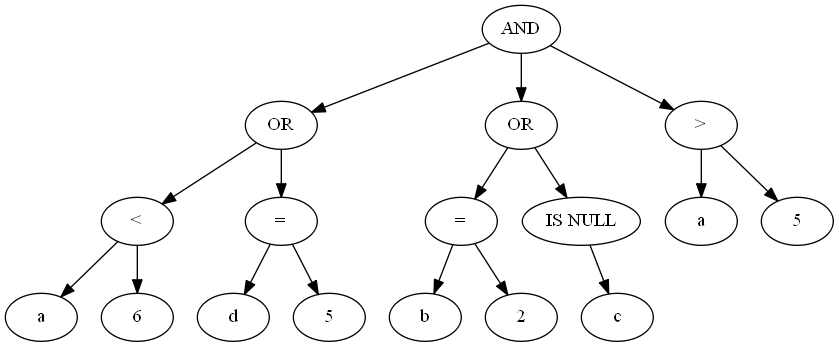
\includegraphics[scale=0.55]{Bilder/sort_zwischen4.png}
\caption{Sortierbeispiel: Ende des Sortierens}
\label{fig:sort_zwischen4}
\end{figure}

Ist das Sortieren abgeschlossen, entfernen wir noch unnötige Duplikate. Haben die Operatoren \verb|AND| oder \verb|OR| zwei gleiche Operanden $o_1,o_2$, die äquivalent sind ($T(o_1) \equiv T(o_2)$), so können wir einen der beiden Operanden streichen. Gleiches gilt für den Operator \verb|OR|. Durch die Sortierung stehen solche Duplikatskandidaten immer nebeneinander. Wir durchsuchen den Baum daher iterativ nach Duplikaten und entfernen diese.

\subsection{GROUP BY / HAVING}

Bisher haben wir den SELECT-, FROM- und WHERE-Teil einer SQL-Anfrage bearbeitet. Anfragen, die einen GROUP BY-Teil enthalten müssen auch nach festen Regeln angepasst werden. Da die Reihenfolge innerhalb dieses Teils unwichtig ist, sortieren wir die Spaltennamen lexikographisch. Die Tupelvariablen sind bereits automatisch benannt nach dem Schema \verb|aN| mit $N\in \{1,2,...\}$ (siehe Unterabschnitt \ref{subsec:from}).

Der HAVING-Teil wiederum ähnelt von seiner Struktur dem WHERE-Teil. Es handelt sich ebenso um einen komplexeren Ausdruck. Wir behandeln daher den HAVING-Teil sowie den WHERE-Teil im Unterabschnitt \ref{subsec:where}.

Nicht wichtig für die einheitliche Anpassung ist, ob die Tabellen bzw. Aggregationsfunktionen im GROUP BY-Teil auch im SELECT-Teil vorkommen. Dies könnte aber auf einen ungewollten Fehler des Lernenden hinweisen. Diese Information wird daher im Preprocessing (siehe Abschnitt \ref{subsec:preprocessing}) mit aufgenommen. 

\subsection{ORDER BY}

Der ORDER BY-Teil kann nicht im Sinne der Standardisierung angepasst werden. Die hier angegebene Reihenfolge kann nicht verändert werden, ohne den Sinn des Ausdruckes zu ändern. Die Anpassung beschränkt sich also auf das Umbenennen der Tupelvariablen, wie es im Unterabschnitt \ref{subsec:from} beschrieben ist.

Interessant für das Preprocessing sind allerdings andere Informationen über ORDER-BY. So merken wir uns, ob die Anfrage ORDER BY-Klauseln mit einem expliziten ASC enthält, da dies unnötig ist.

Weiterhin ist es möglich die Nummer der Spalte, anstatt den Spaltennamen bei der Sortierung anzugeben. Wir ersetzten dabei die Nummer mit dem korrespondierendem Spaltennamen. Wenn in der Aufgabe notiert wurde, dass die Reihenfolge der Spalten egal ist, dann wurden die Einträge unter \verb|SELECT| bereits in Abschnitt \ref{subsec:select} sortiert. Wir müssen also diese Ersetzung vor dieser Sortierung durchführen, da sich sonst die Spaltennummern ändern. Im Programm realisieren wir dies dadurch, dass wir stets die unangetastete Originalanfrage mit abspeichern.

\subsection{Aggregatsfunktionen}

Die Aggregationsfunktionen \verb|MIN()| und \verb|MAX()| benötigen niemals ein \verb|DISTINCT|. Dennoch ist es nicht falsch. Eine Anfrage, die also \verb|DISTINCT| unter diesen Aggregationsfunktionen benutzt, kann dennoch semantisch äquivalent mit der Musterlösung sein. Im Zuge des Standardisierungsprozesses entfernen wir \verb|DISTINCT| innerhalb von \verb|MAX()| und \verb|MIN()|.

Gibt es innerhalb von \verb|COUNT()| kein \verb|DISTINCT| und kann das Argument von \verb|COUNT()| nicht null sein, so ist die Schreibweise \verb|COUNT(attribute)| äquivalent zu \verb|COUNT(*)|. Wir untersuchen daher alle \verb|COUNT()|-Funktionen auf diese Eigenschaften und ersetzen das Argument ggf. zu \verb|*|.

\subsection{Selbstverbunde}

Bevor wir alle Schritte zusammenfassen, möchten wir uns mit Selbstverbunden beschäftigen. Dazu betrachten wir das folgende Beispiel. Dies ist konstruiert und dient nur zur Veranschaulichung eines Problems.

\begin{verbatim}
Musterlösung:
SELECT * FROM emp e, emp f, dept d WHERE e.sal < 1000 AND e.id = f.id

Anfrage des Lernenden:
SELECT * FROM emp e, emp f, dept d WHERE f.sal < 1000 AND e.id = f.id
\end{verbatim}

Wir bemerken, dass beide Anfragen semantisch äquivalent sind. Allerdings prüfen wir das Gehalt in der Musterlösung mit der ersten Tupelvariable und in der Anfrage des Lernenden mit der zweiten Tupelvariable. Unser Programm erkennt daher keine Äquivalenz zwischen beiden Anfragen. Problem ist hierbei der Selbstverbund. Wir können daher im \verb|WHERE|-Teil die Tupelvariablen $e$ und $f$ beliebig tauschen und erhalten immer das gleiche Ergebnis. 

Wir können Selbstverbunde erhalten, indem wir aus einer Anfrage mit Selbstverbund, mehrere Anfragen konstruieren. Dabei permutieren wir für jede erstellte Anfrage die Tabellen unter \verb|FROM| und substituieren dann im \verb|WHERE-, GROUP BY|- und \verb|ORDER BY|-Teil die Tupelvariablen gemäß der jeweiligen Permutation. Um den Prozess zu verdeutlichen, betrachten wir noch einmal unser Beispiel. 

Wir erstellen aus dem \verb|FROM|-Teil eine Liste der Tupelvariablen: \verb|[e, f, d]|. Dann gruppieren wir die Liste, so dass sich alle gleichen Tabellen in einer Gruppe befinden: \verb|[ [e, f], [d] ]|. Nun erstellen wir alle Permutationen, indem alle inneren Gruppen permutiert werden. Danach entfernen wir die Gruppierungen wieder und erhalten die folgenden, permutierten Listen:
\begin{verbatim}
[ [e, f], [d] ]  =>  [ e, f, d ]
[ [f, e], [d] ]  =>  [ f, e, d ]
\end{verbatim}

Auf Grundlage dieser Listen, erzeugen wir Substitutionen. Wir substituieren jeweils ein Element aus der Originalliste durch ein Element der erzeugten Permutationslisten. In unserem Fall entstehen dann folgende Substitutionen:

\begin{lstlisting}[mathescape]
$\sigma_1$ = [ e/e, f/f, d/d ]
$\sigma_2$ = [ e/f, f/e, d/d ]
\end{lstlisting}

Diese Substitutionen wenden wir nun auf den \verb|WHERE|-Teil unserer Musterlösung an und erhalten:

\begin{lstlisting}[mathescape]
Musterloesung 1 $(\sigma_1)$:
SELECT * FROM emp e, emp f, dept d 
WHERE e.sal < 1000 AND e.id = f.id 

Musterloesung 2 $(\sigma_2)$: 
SELECT * FROM emp e, emp f, dept d 
WHERE f.sal < 1000 AND f.id = e.id 

Musterloesung 2 ($\sigma_2$, sortiert): 
SELECT * FROM emp e, emp f, dept d 
WHERE f.sal < 1000 AND e.id = f.id 
\end{lstlisting}
\begin{verbatim}
Anfrage des Lernenden (unverändert):
SELECT * FROM emp e, emp f, dept d WHERE f.sal < 1000 AND e.id = f.id
\end{verbatim}


Zu beachten ist, dass in Anfrage 2 auch das Verbundskriterium getauscht wird. Aufgrund unserer Sortierordnung, fällt diese Vertauschung dann aber nicht mehr auf, wie wir in Anfrage 3 sehen können. Weiterhin beobachten wir, dass die unveränderte Anfrage des Lernenden nun auf eine der entstandenen Musterlösungen passt.

\subsection{Abschluss}

Wir fassen die einzelnen Schritte noch einmal kurz zusammen: Zunächst haben wir den \verb|FROM|-Teil der Anfrage vereinheitlicht, indem wir einheitliche Tupelvariablen erzeugt haben, nachdem alle Tabellen im \verb|FROM|-Teil lexikographisch sortiert wurden. Alle neu erzeugten Tupelvariablen wurden im Rest der Anfrage korrekt eingesetzt bzw. ersetzt. Finden wir in diesem Schritt im \verb|FROM|-Teil bereits zwei gleiche Tabellen mit unterschiedlichen Tupelvariablen, so könnte ein Selbstverbund dadurch entstehen. Um Mehrdeutigkeiten zu vermeiden, erzeugen wir eine Kopie der vorliegenden Anfrage und vertauschen die gleichen Tabellennamen im \verb|FROM|-Teil. Wir erhalten somit für jeden Selbstverbund einen zusätzlich zu untersuchenden Baum. Am Ende prüfen wir, ob einer dieser Bäume syntaktisch äquivalent ist mit einem der erzeugen Bäume, der zweiten Anfrage. Danach haben wir den \verb|WHERE|-Teil bearbeitet. Wir haben zunächst unnötige Klammern entfernt und die Formeln in die KNF überführt. Danach haben wir einfache syntaktische Varianten ersetzt, um eine einheitlichere Darstellung zu erhalten. Dazu gehörte es auch Unteranfragen aufzulösen oder, wenn nicht möglich, in eine \verb|EXISTS|-Unteranfrage zu überführen. Einer der letzten Schritte war das Behandeln der Vielfalt der Operatoren. Hier haben wir für alle nicht-kommutativen Operatoren ihre alternativen Schreibweisen konjunktiv-verknüpft mit in die Formel aufgenommen. Nach diesem Schritt müssen wir nun die KNF wiederherstellen, da diese durch hinzufügen von \verb|AND|-Knoten zerstört sein kann. Schlussendlich haben wir den gesamten \verb|WHERE|-Teil sortiert, um eine Vereinheitlichung zu erreichen. Anschließend sortierten wir die Attribute innerhalb des \verb|GROUP BY|-Statements lexikographisch. Der Ausdruck im \verb|HAVING|-Teil, wurde genauso behandelt wie der Ausdruck des \verb|WHERE|-Teils. 

\section{Weitere Betrachtungen}

\subsection{JOINS}
\label{subsec:joins}

Wir betrachten in diesem Abschnitt die Behandlung von JOINs. Wir untersuchen wie wir die unterschiedlichen Verbundstypen vereinfachen oder in eine einheitliche Form umwandeln können. Weiterhin interessiert uns die Frage, wie wir unnötige JOINs erkennen können. Wir diskutieren in wie weit eine automatische Entfernung von unnötigen JOINs Sinn macht und wie das Feedback für den Lernenden aussehen kann.

Vorab möchten wir bemerken, dass die Standardisierung und Eliminierung von JOINs eine fortgeschrittene Strategie darstellt. Diese wird daher nicht im Prototypen auftauchen.

\subsubsection*{CROSS JOIN}

Ein \verb|CROSS JOIN| zweier Relationen liefert das kartesische Produkt beider zurück. Das Schlüsselwort \verb|CROSS JOIN| unter \verb|FROM| markiert diesen. Das Schlüsselwort kann allerdings auch weggelassen und durch ein Komma ersetzt werden. Um eine einheitliche Darstellung dieses Verbundtypes zu gewährleisten, werden wir das Schlüsselwort \verb|CROSS JOIN| ersetzen, so dass wir eine Liste von Tabellen unter \verb|FROM| erhalten, welche mit Komma getrennt sind.

\subsubsection*{NATURAL JOIN}

Ein natürlicher Verbund (NV) ist ein Verbund im \verb|FROM|-Teil. Er wird markiert durch die Schlüsselworte \verb|NATURAL JOIN|. Der Verbund zweier Relationen erfolgt über die Attribute, die in beiden Relationen die gleiche Bezeichnung haben. Gibt es keine solchen Attribute, ist das Ergebnis das kartesische Produkt beider Relationen.

Es gibt zwei Möglichkeiten, wie natürliche Verbunde standardisiert werden können. Die erste Möglichkeit besteht darin,   alle Verbundskriterien zu durchsuchen. Stellt man fest, dass die Attribute bei einem Verbundskriterium identisch sind, so handelt es sich um einen natürlichen Verbund. Man könnte diese Kriterien nun streichen und mit dem Schlüsselwort \verb|NATURAL JOIN| explizit kennzeichnen, dass es sich um einen NV handelt. Ein erstes Problem bei dieser Methode ist, dass die Formel unter \verb|WHERE| sehr komplex sein kann. Es ist generell unentscheidbar, ob Verbundskriterien in der Formel auftauchen, da sie auch transitiv-impliziert sein können. Ein zweites Problem ist das folgende Szenario: Angenommen der Lernende L reicht eine Lösung ein, die einen natürliche Verbund zwischen \verb|t1| und \verb|t2| explizit enthält. Weiterhin gibt es kein namensgleiches Attribut in \verb|t1| und \verb|t2|, so dass der natürliche Verbund im Prinzip ein kartesisches Produkt ist. In der Musterlösung stehen \verb|t1| und \verb|t2| nur unter \verb|FROM|, um eben dieses Produkt zu erzeugen. Die Methode 1 würde nun gar keine Anpassung machen, da es kein Kriterium für einen potentiellen natürlichen Verbund in der Anfrage des L findet. Als Folge können wir die beiden Anfragen nicht matchen, obwohl beide das gleiche tun.

Die zweite Möglichkeit besteht darin explizite natürliche Verbunde umzuschreiben, indem wir das Schlüsselwort \verb|NATURAL JOIN| entfernen und beide Relationen nach gleichnamigen Attributen durchsuchen. Der Vorteil gegenüber der  ersten Methode ist, dass wir immer entscheiden können, ob zwei endliche Relationen zwei gleichnamige Attribute besitzen. Haben wir dann solche Attribute gefunden, so fügen wir diese explizit als Verbundskriterien ein. Haben wir keine solche Kriterien gefunden, handelt es sich um ein kartesisches Produkt. Wir fügen in diesem Fall die zweite Tabelle unter \verb|FROM| hinzu und eliminieren das Schlüsselwort \verb|NATURAL JOIN|.

Beide Methoden haben einen gewissen Aufwand zu bewältigen, allerdings haben wir schon bemerkt, dass Methode 1 unentscheidbare Probleme mit sich bringt. Bei Methode 1 müssen wir alle Verbundskriterien durchsuchen. Die Formel kann komplex sein und außerdem ist durch mögliche transitiv-implizierten Gleichungen nicht entscheidbar, ob Verbundskriterien existieren. In Methode 2 müssen wir zwei Relationen paarweise nach gleichnamigen Attributen durchsuchen, was bei endlichen Relationen immer entscheidbar ist.
Aus diesen Gründen entscheiden wir uns für Methode 2. Weil wir den \verb|NATURAL JOIN| unter \verb|FROM| auflösen, schreiben wir diesen als \verb|INNER JOIN| unter die \verb|WHERE|-Bedingung, wie das  Beispiel \ref{bsp:natjoin} zeigt (angenommen \textit{table1} und \textit{table2} haben beide eine gleichnamige Spalte namens \textit{id}).

\begin{figure}[H]
\begin{verbatim}
Vorher:
SELECT t1.col1 FROM table1 t1 NATURAL JOIN table2 t2

Danach:
SELECT t1.col1 FROM table1 t1, table2 t2 WHERE t1.id=t2.id
\end{verbatim}
\caption{Beispiel: Standardisierung eines natürlichen Verbundes}
\label{bsp:natjoin}
\end{figure}

\subsubsection*{OUTER JOIN}

Bei einem \verb|OUTER JOIN| unterscheiden wir zwischen einem \verb|LEFT OUTER JOIN| und einem \\\verb|RIGHT OUTER JOIN|. Ein \verb|FULL OUTER JOIN| ist die Verbindung, also ein \verb|UNION| vom linken und rechten \verb|OUTER JOIN|. Wir betrachten daher exemplarisch zunächst den \verb|LEFT OUTER JOIN|, da sich die Betrachtungen dann äquivalent auf den rechten Verbund und damit auf den \\\verb|FULL OUTER JOIN| übertragen lassen.

Zunächst ist zu klären, wie der \verb|OUTER JOIN| alternativ formuliert werden kann. Dazu gehen wir kurz darauf ein, was ein \verb|LEFT OUTER JOIN| genau macht. Die ``linke'' Tabelle wird vollständig aufgeführt. Dann wird jeder Eintrag der Tabelle sukzessive betrachtet. Gibt es im aktuellen Eintrag einen Verbundpartner in der ``rechten'' Tabelle (vorgegeben durch das Verbundskriterium), dann werden die Daten der ``rechten'' Tabelle an den Eintrag angehangen. Ist dies nicht der Fall, wird der Eintrag mit \textit{NULL} Einträgen aufgefüllt. 

Um die Umwandlung eines \verb|LEFT OUTER JOIN| zu demonstrieren, betrachten wir folgendes Beispiel:

\begin{figure}[H]
\begin{verbatim}
SELECT e.empno, e.job, d.dname 
FROM dept d 
LEFT JOIN emp e ON e.deptno = d.deptno 
WHERE d.loc <> 'CHICAGO'
ORDER BY e.empno
\end{verbatim}
\caption{OUTER JOIN Beispiel}
\end{figure}

Wir haben also zwei verschiedene Mengen von Einträgen. Zum einen Einträge, die einen Verbundpartner besitzen und zum Anderen Einträge, die keinen solchen Partner haben. Anbieten würde sich an dieser Stelle die Verwendung einer Vereinigung (\verb|UNION|) der beiden eben genannten Mengen. Dabei ist die Umwandlung in ein solches Statement mit einem \verb|UNION| keinesfalls trivial und unterliegt einigen Einschränkungen, die wir im Folgenden behandeln werden. 

Ziel ist es also zwei SQL-Anfragen zu formulieren, die jeweils für die oben genannten Mengen stehen. Anschließend werden diese Mengen mit einem \verb|UNION| verbunden.

Für die SQL-Anfrage, welche die Menge der Verbundpartner angibt, übernehmen wir zunächst den \verb|SELECT|-Teil. Die zwei Tabellen, die am Verbund beteiligt sind werden im \verb|FROM|-Teil nun als \verb|CROSS JOIN| aufgeschrieben, also mit Komma getrennt. Der \verb|WHERE|-Teil wird ebenfalls vom gegebenen \verb|OUTER JOIN|-Statement übernommen und durch die Angabe des Verbundskriteriums ergänzt.
Wir erhalten also die folgende Anfrage bezüglich unseres Beispiels:

\begin{figure}[H]
\begin{verbatim}
SELECT e.empno, e.job, d.dname 
FROM dept d, emp e
WHERE d.deptno = e.deptno
AND d.loc <> 'CHICAGO'
ORDER BY e.empno
\end{verbatim}
\caption{OUTER JOIN Umwandlung, 1. Teil}
\end{figure}

Nun muss noch die Teilmenge aller Tupel hinzugefügt werden, die keinen Verbundpartner haben. Wir übernehmen zunächst wieder den \verb|SELECT|-Teil der Ursprungsanfrage, ersetzen aber alle Spaltennamen der ``rechten'' Tabelle mit \verb|NULL|, weil diese Werte aufgrund fehlender Verbundpartner nicht belegt sind. Diese Ersetzungen müssen ebenso im \verb|WHERE|-Teil stattfinden. Die rechte Tablle wird aus dem \verb|FROM|-Teil gestrichen. Nun passen wir den \verb|WHERE|-Teil an. Hier könnte man auf die Idee kommen mit einem \verb|NOT IN| Semijoin zu prüfen, dass auch nur Tupel ohne Verbundpartner aufgenommen werden. Erlaubt  das Verbundskriterium in der ``linken'' Tabelle \verb|NULL|-Werte, so würden diese Einträge nicht erscheinen. Bei einem \verb|LEFT OUTER JOIN| sind diese Tupel aber mit erfasst. Es bietet sich daher eine \verb|NOT EXISTS|-Unterabfrage an. 

\begin{figure}[H]
\begin{verbatim}
SELECT NULL, NULL, d.dname
FROM dept d 
WHERE NOT EXISTS(
    SELECT 1 FROM emp e WHERE d.deptno = e.deptno )
AND d.loc <> 'CHICAGO'
ORDER BY e.empno
\end{verbatim}
\caption{OUTER JOIN Umwandlung, 2. Teil}
\end{figure}

Nun müssen beide Anfragen mit einem \verb|UNION ALL| verknüpft werden. Dabei müssen wir das \verb|ORDER BY|-Statement ausklammern, da dieses erst auf dem Datensatz, der mit \verb|UNION ALL| erzeugt wurde, ausgeführt wird. Unser Endergebnis bezogen auf unser Beispiel lautet also:

\begin{figure}[H]
\begin{verbatim}
SELECT e.empno, e.job, d.dname FROM dept d, emp e
WHERE d.deptno = e.deptno AND d.loc <> 'CHICAGO'
    UNION ALL
SELECT NULL,NULL,d.dname FROM dept d 
WHERE NOT EXISTS(
  SELECT 1 from emp e where d.deptno = e.deptno)
AND d.loc <> 'CHICAGO'
ORDER BY empno
\end{verbatim}
\caption{OUTER JOIN Umwandlung, finaler Schritt}
\end{figure}

Bei diesem Vorgehen kann es passieren, dass bei bestimmten SQL-Anfragen nach der Umwandlung in einen \verb|OUTER-JOIN| klar wird, dass dieser äquivalent zu einem \verb|INNER JOIN| ist. Dazu betrachten wir das Beispiel in Abbildung \ref{fig:outer_s1}.

\begin{figure}[H]
\begin{verbatim}
SELECT e.empno, e.job, d.dname 
FROM dept d 
LEFT JOIN emp e ON e.deptno = d.deptno 
WHERE e.sal > 2000
ORDER BY e.empno
\end{verbatim}
\caption{OUTER JOIN: Spezialfall}
\label{fig:outer_s1}
\end{figure}

Wie wir sehen, taucht im \verb|WHERE|-Teil ein Attribut der ``rechten'' Tabelle auf, was formal zu der Anfrage führen würde, die wir in Abbildung \ref{fig:outer_s2} erkennen.

\begin{figure}[H]
\begin{verbatim}
SELECT e.empno, e.job, d.dname FROM dept d, emp e
WHERE d.deptno = e.deptno AND e.sal > 2000
    UNION ALL
SELECT NULL,NULL,d.dname FROM dept d 
WHERE NOT EXISTS(
  SELECT 1 from emp e where d.deptno = e.deptno)
AND NULL > 2000
\end{verbatim}
\caption{OUTER JOIN: Spezialfall Endergebnis}
\label{fig:outer_s2}
\end{figure}

Wie man sieht, kann die Bedingung \verb|NULL > 2000| nie erfüllt werden, außer es handelt sich um einen Syntaxfehler. Daher muss die zweite Anfrage komplett gestrichen werden und wir erhalten die Anfrage in Abbildung \ref{fig:outjoinspez2}, was nun ein üblicher \verb|INNER JOIN| ist.

\begin{figure}[H]
\begin{verbatim}
SELECT e.empno, e.job, d.dname FROM dept d, emp e
WHERE d.deptno = e.deptno AND e.sal > 2000
\end{verbatim}
\caption{OUTER JOIN: Spezialfall}
\label{fig:outjoinspez2}
\end{figure}


Eine Besonderheit stellt das \verb|GROUP BY|-Statement dar. Dies wurde nicht im Beispiel benutzt, daher betrachten wir nun im Folgenden, wie damit zu verfahren ist:

Wird in der \verb|OUTER JOIN|-Abfrage nach mindestens einem Attribut der ``rechten'' Tabelle gruppiert, so müssen wir die Gruppierung in eine weitere Anfrage schachteln. Dazu bauen wir die Anfrage, wie oben beschrieben, auf und streichen zunächst das \verb|GROUP BY|-Statement. Aggregationsfunktion \textit{agg(x)} werden ersetzt durch \textit{x}. Um die dann entstandene, mit \verb|UNION ALL| verknüpfte SQL-Anfrage A schachteln wir eine weitere Anfrage B. Der \verb|SELECT|-Teil von B entspricht dem, der ursprünglichen \verb|OUTER JOIN|-Anfrage. Der \verb|FROM|-Teil von B entspricht der konstruierten Anfrage A. Einen \verb|WHERE|-Teil von B gibt es nicht, da dieser bereits in der Anfrage A eingearbeitet wurde. Ergänzt wird die Anfrage B mit dem \verb|GROUP BY|- und \verb|ORDER BY|-Statement der Ursprungsanfrage.

Existiert im \verb|GROUP BY|-Teil der Originalanfrage kein Attribut der ``rechten'' Tabelle, ist die eben genannte Schachtelung nicht notwendig. Es reicht hier aus den \verb|GROUP BY|-Teil einfach in die konstruierten Teilanfragen mit einzubeziehen. Grund dafür ist, dass wir disjunkte Gruppierungen in beiden Anfragen erhalten und diese ohne Probleme mit \verb|UNION ALL| vereinigen können.

Dies waren alle notwendigen Schritte, um einen \verb|LEFT OUTER JOIN| äquivalent in eine komplexe Anfrage mit \verb|UNION ALL| und Semijoins zu überführen. Zu Bemerken ist an dieser Stelle, dass ein \verb|RIGHT OUTER JOIN| entsprechend behandelt wird, nur mit umgekehrten Seiten. Einen \verb|FULL OUTER JOIN| erhalten wir durch ein \verb|UNION| vom \verb|LEFT OUTER| und \verb|RIGHT OUTER JOIN|. 

Nach dieser Betrachtung müssen wir jedoch feststellen, dass die Umwandlung eines \verb|OUTER JOIN| recht vielschichtig und aufwendig ist. Es ist zwar möglich diesen äquivalent umzuformen, allerdings wird der Ausdruck dadurch enorm aufgebläht. Weiterhin funktioniert diese Umwandlung nur in eine Richtung problemlos, nämlich vom \verb|JOIN| zum \verb|UNION|-Ausdruck. Umgekehrt ist es sehr aufwendig festzustellen, ob ein \verb|UNION ALL| auch ein \verb|OUTER JOIN| ist, da man zum Beispiel Vergleiche mit \verb|NULL|-Werten (wie im Beispiel: \verb|NULL > 2000|) gewöhnlich nicht ausschreibt oder sogar entfernt. Unser Programm soll \verb|OUTER JOIN| daher nicht in einen \verb|UNION ALL|-Ausdruck umwandeln. Wir beschränken uns in der Praxis also darauf, einen \verb|OUTER JOIN| unter \verb|FROM| rein syntaktisch zu erkennen und nicht umzuwandeln. 

Es sei an dieser Stelle auf die Arbeit \cite{outer2inner} verwiesen, in der ein Verfahren vorgestellt wird, welches \verb|OUTER JOIN| äquivalent in \verb|INNER JOIN| umwandelt. Das Verfahren ist komplex und mehrstufig, kann aber mit allen \verb|OUTER JOIN| umgehen. Der entstandene \verb|INNER JOIN| ist allerdings aufgebläht und nicht mehr lesbar, da er künstlich konstruiert ist. Im Rahmen unserer Arbeit interessiert dieser Fakt nur am Rande, im Zuge einer Erweiterung der semantischen Funktionen unseres Programmes, ist dieser Ansatz aber sicherlich erwähnenswert und interessant.

\subsubsection*{INNER JOIN}

Unter einem \verb|INNER JOIN| verstehen wir den Verbund zweier Tabellen unter \verb|FROM|, mit den Schlüsselworten \verb|INNER JOIN|. Ein solcher Verbund kann leicht als \verb|CROSS JOIN| mit Auswahl in der \verb|WHERE|-Bedingung formuliert werden. Dazu entfernen wir den \verb|INNER JOIN| aus dem \verb|FROM|-Teil und erzeugen einen \verb|CROSS JOIN|. Die Verbundbedingungen werden unter \verb|WHERE| eingefügt.

Ein explizit aufgeschriebener \verb|INNER JOIN| kann auch ein \verb|NATURAL JOIN| sein. Da wir solche Verbunde aber auch als \verb|CROSS JOIN| aufschreiben wollen (siehe oben), müssen wir diesen Spezialfall nicht gesondert betrachten. Das folgende Beispiel soll die Umwandlung von \verb|INNER JOIN| verdeutlichen:

\begin{figure}[H]
Eingabe:\\
\verb|SELECT * FROM emp e INNER JOIN dept d ON e.deptno.id = d.deptno|\\

Umwandlung:\\
\verb|SELECT * FROM emp e, dept d WHERE e.deptno = d.deptno|\\
\caption{Umwandlung von INNER-JOIN}
\end{figure}


\subsubsection{JOIN-Eliminierung}

Im vorherigem Abschnitt haben wir bereits alle üblichen Verbunde betrachtet und gezeigt, wie wir diese äquivalent umformen können. Wir haben erreicht, dass alle Verbunde unter \verb|FROM| ersetzt wurden zu \verb|CROSS JOIN| mit Auswahlkriterien unter \verb|WHERE|. Wir möchten daher in diesem Abschnitt auf eine Methode verweisen, mit der es möglich ist, überflüssige \verb|INNER JOIN| zu erkennen und zu eliminieren.

Die Methode selbst ist detailliert in \cite{joinelem2} beschrieben und würde den Rahmen dieser Arbeit überschreiten. Daher wollen wir hier nur ein Beispiel betrachten und es mit der Methode bearbeiten, um zu sehen was diese leisten kann.

Der Algorithmus aus \cite{joinelem2} findet redundante Verbunde mit Hilfe von referentiellen Integritätsbedingungen (RI). Dann folgt die Entfernung einer Relation bei dem der Verbund aus Tabellen besteht, die durch eine RI-Bedingung verbunden sind (nachfolgend als RI-Joins bezeichnet) und bei der die Tabelle, die den Primärschlüssel enthält nur im Join referenziert wird. Ein RI-Join besteht natürlicherweise aus einem Primärschlüssel- und einem Fremdschlüsselattribut.

Als visuelles Hilfsmittel verwendet das Verfahren sogenannte Joingraphen $G=(V,E)$. Die Knotenmenge $V$ besteht aus Joinattributen. Eine Kante zwischen zwei Knoten $u,v$ existiert genau dann, wenn $u$ und $v$ Teil eines Joinprädikates sind. Handelt es sich bei dem Join um einen RI-Join, also ein Primär-/ Fremdschlüssel Join, dann sind $u,v$ durch eine gerichtete Kante verbunden, wobei der Pfeil dann vom Fremdschlüsselattribut/ Kind zum Primärschlüsselattribut/ Eltern geht. Das Bearbeiten der folgenden Beispielanfrage soll zeigen, wie das Verfahren vorgeht. Die Datenbankschemata sind dem TCP-H entnommen und in \cite{partsubdb} zu finden.

\begin{lstlisting}[mathescape]
SELECT ps.partkey, avg(ps.supplycost)
FROM   supplier s, partsupp ps, customer c, orders o
WHERE  s.suppkey = ps.suppkey 
AND    s.suppkey = c.custkey
AND    c.custkey = o_custkey
AND    o.totalprice >= 100
GROUP BY ps.partkey
\end{lstlisting}

Wir erzeugen zunächst den ersten Joingraphen $G_1$, indem wir jede Joinbedingung als verbundenes Paar in den Graphen einfügen:

\begin{figure}[H]
\centering
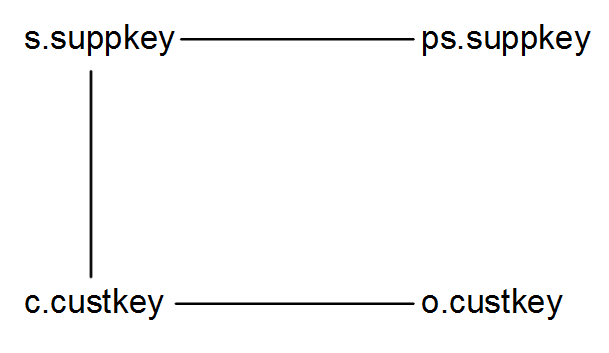
\includegraphics[scale=0.4]{Bilder/joinelem_g1.png}
\caption{$G_1$}
\end{figure}

Wir weisen die RI-Joins aus, in dem wir sie als gerichtete Kanten markieren. Weiterhin fügen wir nun alle transitiv-implizierten Joins als nicht RI-Joins hinzu, also als ungerichtete Kanten, und erhalten damit $G_2$:

\begin{figure}[H]
\centering
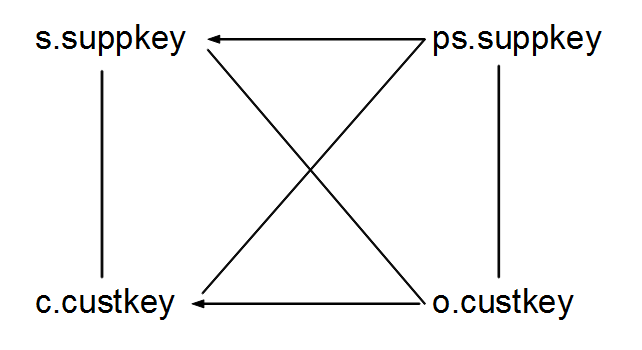
\includegraphics[scale=0.4]{Bilder/joinelem_g2.png}
\caption{$G_2$}
\end{figure}

Im letzten Schritt gehen wir alle Knoten sukzessive durch. Da jeder Knoten ein Attribut repräsentiert, prüfen wir, ob das repräsentierte Attribut in einem Nicht-Join Prädikat unter \verb|WHERE|, im \verb|GROUP BY|- oder im \verb|SELECT|-Teil vorkommt. Falls ja, ersetzen wir das Attribut mit einem Attribut eines Verbundpartners, der noch im Graphen existiert. Dann eliminieren wir den Knoten und alle zugehörigen Kanten. In unserem Beispiel kommt weder \verb|s.suppkey| noch \verb|c.custkey| in den genannten Teilen der Anfrage vor und damit können wir diese Entfernen ohne Attributsreferenzen ersetzen zu müssen. Wir löschen diese Attribute aus $G_2$ und erhalten $G_3$ mit nur noch einem, notwendigen Join:

\begin{figure}[H]
\centering
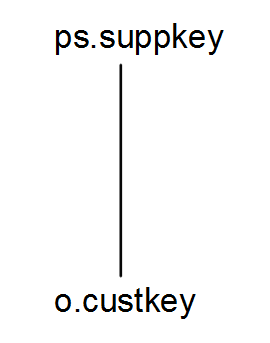
\includegraphics[scale=0.4]{Bilder/joinelem_g3.png}
\caption{$G_3$}
\end{figure}

Wir erhalten also folgende SQL-Anfrage:

\begin{lstlisting}[mathescape]
SELECT ps.partkey, avg(ps.supplycost)
FROM   partsupp ps, orders o
WHERE  o.custkey = ps.suppkey 
AND    o.totalprice >= 100
GROUP BY ps.partkey
\end{lstlisting}


%\section{Komplexität von SQL-Anfragen}

%Durch Standardisierung zweier SQL-Abfragen \verb|query1| und \verb|query2| können wir durch einen syntaktischen Vergleich prüfen, ob es uns möglich war, beide gegeneinander zu matchen. Unabhängig vom Ergebnis dieses Matchings ist für den Lernenden wichtig, wie nah er an der Musterlösung dran war. Folgende Szenarien sind dabei denkbar. 
%
%Im ersten Szenario konnte die SQL-Anfrage des Lernenden nicht mit der SQL-Anfrage der Musterlösung gematcht werden. Der Lernende benötigt nun ein Feedback um seine Fehler zu erkennen und um letztendlich einen neuen Lösungsvorschlag zu machen. 
%
%In einem zweite Szenario konnte die SQL-Anfrage des Lernenden gematcht werden. Während des Standardisierungsprozesses seiner Anfrage, kann es aber sein, dass unnötige Klauseln entfernt wurden. In einem solchen Fall ist es von Interesse dem Lernenden mitzuteilen, dass seine Lösung noch nicht perfekt (im Sinne der Musterlösung) ist. 
%
%Wir wollen im Folgenden nun Kriterien von Metainformationen festlegen. Diese Metainformationen der zwei Anfragen sollen dann jeweils miteinander verglichen werden. Finden wir bei einem solchen Vergleich Unstimmigkeiten in der Anzahl der jeweiligen Informationen, muss dies dem Lernenden mitgeteilt werden.



%\section{Alternativer Ansatz: Elementare Transformationen}

%Der nun vorgestellte Ansatz stellt eine Alternative zur >>Anpassung durch Standardisierung<< dar. Beide %Ansätze haben ähnliche Ideen, sind jedoch in ihrer Umsetzung verschieden. Beim Ansatz der Standardisierung %haben wir zunächst eine SQL-Anfrage genommen und standardisiert. Dies geschah völlig unabhängig zu der zu %vergleichenden, zweiten SQL-Anfrage. Es wurden gewisse allgemeine Regeln aufgestellt und nach diesen wurde jede SQL-Anfrage behandelt und angepasst. Der eigentliche Vergleich geschah dann aufgrund eines Vergleichs der standardisierten Anfragen und dem Vergleich von Metadaten (Anzahl Joins, Anzahl atomarer Formeln, etc.). Ein Nachteil von diesem Ansatz ist, dass wir für jedes mögliche Konstrukt in der SQL-Anfrage auch Regeln im System haben, damit wir jene Konstrukte auch anpassen und standardisieren können. Außerdem findet der Vergleich erst im allerletzten Schritt statt.%
%
%Die >>Anpassung durch elementare Transformationen<< stellt einen intuitiven Ansatz vor. Wir versuchen hier per Backtracking konkret eine Lösung der anderen anzugleichen. Damit haben wir einen konkreten Unterschied zum bisherigen Ansatz. Wir vergleichen die Lösung direkt und umgehen die Vorverarbeitungen. Im Wesentlichen geben wir also ganz allgemeine Regeln an und in jedem Schritt versuchen wir durch Anwendung dieser Regeln die SQL-Anfrage so anzupassen, dass sie auf unsere zu vergleichende Anfrage passt.



\subsection{Unnötiges DISTINCT}

Eine interessante Frage ist, ob ein \verb|DISTINCT| wirklich notwendig ist. Dies ist natürlich wichtig für den Vergleich zweier SQL-Anfragen. In \cite{brass2} wurde im Rahmen des SQLLint-Projektes bereits in dem Prototypen ein Checker eingebaut, der prüft, ob \verb|DISTINCT| wirklich notwendig ist. Aber auch im Rahmen dieser Arbeit ist es notwendig zu wissen, ob das \verb|DISTINCT| notwendig ist. 

Eine erste Idee ist es, die Musterlösung auf ein vorhandenes \verb|DISTINCT| zu prüfen. Allerdings kann es Fälle geben, in denen man anstatt eines \verb|DISTINCT| eine \verb|EXISTS|-Unterabfrage benutzt und daher benötigen wir einen Ansatz, der unabhängig von der Musterlösung entscheidet, ob ein \verb|DISTINCT| notwendig ist.  Im Folgenden stellen wir daher einen Algorithmus vor, der erkennt, ob die Lösung Duplikate enthalten kann oder nicht. Das allgemeine Frage, ob ein \verb|DISTINCT| notwendig ist, ist unentscheidbar. Deswegen prüft der nachfolgende Algorithmus die hinreichende Bedingung für ein unnötiges \verb|DISTINCT|. Das bedeutet, dass wenn der Algorithmus sagt "`ja, \verb|DISTINCT| ist unnötig"', können wir sicher sein, dass es tatsächlich unnötig ist. Sagt der Algorithmus allerdings "`nein"' bedeutet dies nicht notwendigerweise, dass das \verb|DISTINCT| wirklich unnötig ist. 

Der Algorithmus ist nicht in unserem Programm implementiert. Wir beschreiben ihn aber im Folgenden so, dass er in einer Überarbeitung ohne Probleme integriert werden könnte. Der Algorithmus müsste dann in jedem Fall nach der Umwandlung des \verb|WHERE|-Teils in die KNF erfolgen, da dies eine Voraussetzung für den Algorithmus ist.

\subsection{Verbale Beschreibung}

Es sei $\mathcal{K}$ die Menge von Attributen, die für eine Ausgabezeile eindeutig definiert sind. Wir initialisieren diese Menge daher mit allen Ausgabespalten unter \verb|SELECT|. Ziel des Algorithmus ist es, für jede Tabelle unter \verb|FROM| einen Schlüssel zu haben, der sich in $\mathcal{K}$ befindet. Ist dies der Fall, so wissen wir sicher, dass keine Duplikate auftreten können, da jede Spalte durch ihren Schlüssel eindeutig identifiziert wird. 

Wir fügen der Menge $\mathcal{K}$ zunächst alle Attribute A hinzu, wenn A an eine Konstante gebunden ist, also wenn im \verb|WHERE|-Teil $A=c$ oder $c=A$ auftaucht. Dabei gehen wir davon aus, dass unsere \verb|WHERE|-Formel eine Konjunktion ist. Das deckt sich gut mit unserem Programm, da wir eine KNF erzeugen.

Danach fügen wir alle Attribute $B$ der Menge $\mathcal{K}$ hinzu, wenn $B$ mit einem Attribut aus unserer Menge übereinstimmt, also $A=B$ und $A\in\mathcal{K}$. Haben wir nun einen Schlüssel einer Tupelvariable in $\mathcal{K}$, so ist klar, dass Ausgabezeilen für diese Tupelvariable immer eindeutig bestimmt sind und wir fügen alle Attribute dieser Tupelvariable hinzu. Diesen Prozess wiederholen wir solange bis sich $\mathcal{K}$ nicht mehr ändert. 

Haben wir kein \verb|GROUP BY|-Statement, dann prüfen wir, ob von jeder Tupelvariable ein Schlüssel in $\mathcal{K}$ enthalten ist. Haben wir allerdings ein \verb|GROUP BY|-Statement so prüfen wir, ob alle \verb|GROUP BY|-Spalten in $\mathcal{K}$ enthalten sind.

Der folgende Algorithmus ist \cite{sql1folien} entnommen.

\subsection{Algorithmus}

Es sei unsere SQL-Anfrage der Form:

\begin{lstlisting}[mathescape]
SELECT $t_1$, ..., $t_k$
FROM $R_1\ X_1$, ..., $R_n\ X_n$
WHERE $\varphi$
\end{lstlisting}

Es sei $X=\{X_1, ..., X_n\}$ die Menge aller Tupelvariablen. Es sei $G=\{G_1, ..., G_m\}$ die Menge aller \verb|GROUP BY|-Spalten.

Die einzelnen Attribute $t_i$ haben die Form $t = X.k$. Dabei ist $X$ eine Tupelvariable und $k$ ein Attribut. Wir bezeichnen die Menge aller $t_i$ mit $\mathcal{K}=\{t_1,...,t_k\}$.

\begin{lstlisting}[mathescape]
$\mathcal{K}$ = $\mathcal{K}\ \cup$ {A}, wenn $A=c$ als Konjunktion in WHERE auftaucht
do 
  $\mathcal{K'}$ = $\mathcal{K}$
  $\mathcal{K'}$ = $\mathcal{K'}\ \cup$ A, wenn $A=B\in$ WHERE-Bedingung und $B\in\mathcal{K}$
  $\mathcal{K'}$ = $\mathcal{K'}\ \cup$ S mit $S=\{b\in X\}$, wenn $t\in \mathcal{K'}$ ein Schluessel ist und t=X.k
while ($\mathcal{K}\ \neq\ \mathcal{K'}$)

if not Anfrage hat GROUP BY Statement:
  foreach $x\in X$ do
    if not ($\exists k\in \mathcal{K'}$ mit $k$ ist Schluessel von $x$)
      break and return NO
    endif
  done

if Anfrage hat GROUP BY Statement:
  foreach $g\in G$ do
    if $g\notin \mathcal{K'}$
      break and return NO
    endif
  done

return YES
\end{lstlisting}


\section{SQL-Anfragen auf externen Datenbanken}
\label{sec:externalDBS}

Bis jetzt haben wir verschiedene Methoden und Ansätze diskutiert, die sich auf das Erfüllen der hinreichenden Bedingung einer semantischen Äquivalenz konzentriert haben. In den vorherigen Abschnitten dieses Kapitels haben wir festgestellt, dass eine, durch Überführung, erhaltene syntaktische Äquivalenz zweier SQL-Anfragen automatisch deren semantische Äquivalenz bedeutet. Wie eingangs erwähnt, ist das Problem, zwei SQL-Anfragen auf semantische Äquivalenz zu prüfen, im Allgemeinen nicht entscheidbar. Aus diesem Grund kann es passieren, dass unsere bisher erarbeiteten Methoden, bei einigen, semantisch äquivalenten, Anfragen keinen Erfolg bringen. Die Anfragen sind dann semantisch äquivalent, aber wir können sie nicht durch unsere Methoden aneinander anpassen. 

Für diese Art von Anfragen prüfen wir eine notwendige Bedingung der semantischen Äquivalenz zweier Anfragen. Für diesen Schritt benötigen wir echte Daten für das, jeweils gegebene, Datenbankschema. Wir führen sowohl die Musterlösung als auch die Lösung des Lernenden auf einer Datenbank mit realen Daten aus. Wir vergleichen dann die zurückgelieferten Tupel. Unterscheiden sich diese, dann wissen wir, dass die beiden Anfragen nicht semantisch äquivalent sein können. Dabei würde der Unterschied in beiden Antwortmengen das Gegenbeispiel zur Äquivalenz darstellen.

Sind die Antwortmengen identisch für alle vorhandenen Datenbankzustände, ist dies kein sicheres Zeichen dafür, dass die Anfragen semantisch äquivalent sind, da dies nur das notwendige Kriterium, nicht aber ein hinreichendes Kriterium ist. Haben wir also zwei SQL-Anfragen, deren semantische Äquivalenz weder durch Standardisierung nachgewiesen noch durch Tests auf realen Daten widerlegt werden konnte, so wissen wir nicht, ob diese Anfragen sicher äquivalent sind oder nicht. Wir geben dem Lernenden dann das Feedback, dass seine Lösung eventuell richtig oder falsch ist. Auch muss der Dozent, oder andere Berechtigte, über solche Lösungen informiert werden. Die berechtigte Person kann dann entscheiden, ob die Lösung eine weitere Musterlösung darstellt, oder nicht korrekt ist.

Im Detail gibt es allerdings einige Feinheiten zu beachten, wenn man die Anfragen auf konkreten Datenbanken mit echten Daten ausführen will. Im Folgenden werden wir diese Feinheiten erläutern und mögliche Probleme disktuieren.

\subsection{Unterschiedliche DBMS}

Obwohl es, in gewissen Abständen, zur Herausgabe eines Standards für SQL durch die ISO kommt, unterscheiden sich die existierenden DBMS bei der Handhabung und Implementation von SQL-Features. Die aktuellste Version des SQL-Standards ist zur Zeit: SQL:2008. Die verschiedenen Hersteller variieren diesen Standard allerdings, durch Entfernen oder Hinzufügen von Funktionalitäten. Diese Änderungen sind sowohl in der Data Definiton Langauge (DDL), der Data Manipulation Language (DML) als auch der Data Control Language (DCL) zu finden. Wir gehen im Folgenden auf einige Unterschiede ein. Da wir im Hinblick auf diese Arbeit gerne unabhängig von den Herstellern verschiedener DBMS sein wollen, ist für uns interessant, welche Schnittmenge von Funktionalitäten alle DBMS gemeinsam haben. Nach heutigem Stand können wir sagen, dass DB2, MSSQL, MySQL, Oracle und Informix mindestens den SQL-92 Entry Level-Standard erfüllen. PostgreSQL hat zusätzlich noch das Konzept der Sichten, erlaubt aber nicht, diese zu aktualisieren (update). Um diese Restriktion zu umgehen, führt PostgreSQL ein, nicht vom Standard vorgesehenes, Konzept von Regeln ein, auf das wir nicht näher eingehen wollen. Ist unsere Anfrage also SQL-92 konform, so können wir diese ohne Probleme auf allen gängigen DBMS ausführen.

Betrachten wir nun ein paar Unterschiede im Detail. Von den, oben genannten, DBMS verstehen nur PostgreSQL, MySQL und Oracle das Schlüsselwort \verb|NATURAL JOIN| unter \verb|FROM|. \verb|FULL JOIN|, also die Vereinigung eines \verb|LEFT OUTER| und \verb|RIGHT OUTER| Join verstehen alle DBMS, bis auf MySQL. Alle DBMS verstehen aber das explizite kartesische  Produkt, \verb|CROSS JOIN|. Dieser Sachverhalt kommt uns entgegen, da wir versuchen im ersten Teil, der Standardisierung, alle Joins als kartesisches Produkt mit Auswahl zu formulieren, falls das möglich ist. Können wir bestimmte Joins nicht umschreiben, kann es zu Laufzeitfehlern kommen, welche später in diesem Kapitel behandelt werden.

Unterschiede in der DDL behandeln wir nicht, da wir uns im Rahmen dieser Arbeit nur mit dem \verb|SELECT|-Statement beschäftigen. Ein wesentlicher Unterschied hierbei besteht in der Sortierung von Werten. Der Standard trifft keine Aussage darüber, wie \verb|NULL|-Werte im Verlgeich zu nicht-\verb|NULL|-Werten sortiert werden sollen. Der Standard beschreibt lediglich die Schlüsselwörter \verb|NULLS FIRST| sowie \verb|NULLS LAST|, um das Verhalten dementsprechend zu erzwingen. In der Implementation haben sich die Hersteller allerdings entscheiden müssen, was im default-Fall zu tun ist. In den Systemen PostgreSQL, DB2 und Oracle werden \verb|NULL|-Werte mit höherer Priorität als nicht-\verb|NULL|-Werte behandelt. Dementsprechend behandeln MSSQL, Informix und MySQL die \verb|NULL|-Werte niedriger, als die nicht-\verb|NULL|-Werte. Bei Oracle tritt zusätzlich die Besonderheit auf, dass ein leerer String identifiziert wird mit einem \verb|NULL|-Wert.

Weitere Unterschiede zwischen den DBMS treten auf in Bezug auf das Schlüsselwort \verb|LIMIT n|, welches bewirkt, dass nur die ersten $n$ Datensätze ausgegeben werden. Lediglich MySQL und PostgreSQL kennen dieses Schlüsselwort. Bei allen anderen DBMS muss diese Anforderung durch Verwendung der \textit{row-number} umgesetzt werden. 

Weitere Unterschiede haben die DBMS bei Verwendung vom \verb|BOOLEAN|-Datentyp, dem \verb|UNIQUE|-Constraint, der Konkatenation von Strings, dem Schlüsselwort \verb|LOCALTIMESTAMP|, der Funktion \verb|SUBSTRING| und dem Datentyp \verb|TIMESTAMP|. Es würde zu weit führen, alle Unterschiede genau zu betrachten. Nachzulesen sind die genauen Unterschiede unter \cite{sqldiff1}.

Wichtig für unsere Arbeit ist, dass wir keine Probleme zu erwarten haben, wenn eine Anfrage SQL-92 Entry-Level konform ist. Sollte dies nicht der Fall sein, werden wir, mit großer Wahrscheinlichkeit, einen Laufzeitfehler oder einen Fehler beim Parsen der Anfrage erhalten.

Haben wir dennoch eine SQL-Anfrage, die nicht von allen DBMS gleichartig verstanden wird, so können wir die Unterschiede mit unserem Programm gut beobachten. Aufgrund der Programmstruktur, die in Kapitel \ref{chap:praxis} erläutert ist, senden wir die Anfrage an alle angeschlossen, externen DBMS. Tritt dabei ein Laufzeitfehler auf, so wird dieser an den Nutzer weitergereicht. So können wir testen, auf welchen DBMS unsere Anfrage ausgeführt werden kann und auf welchen nicht. Weiterhin kann es möglich sein, dass eine Anfrage von keinem der angeschlossenen DBMS verstanden wird. Dann erhält der Nutzer die Fehlermeldungen aller DBMS. Dabei ist es möglich, dass bestimmte DBMS exaktere oder verständlichere Fehlermeldungen liefern als andere und somit wird potentiell das Verständnis der Fehlermeldungen für den Nutzer erhöht.

\subsection{Visualisierung von Ergebnistupeln}

Wir wollen zwei SQL-Anfragen auf einer konkreten Datenbank ausführen. Nun müssen wir die entstandenen Ergebnismengen miteinander vergleichen. Dabei wollen wir in diesem Abschnitt diskutieren wie dies am sinnvollsten Geschehen soll. 

Der erste Ansatz besteht darin, beide Ergebnismengen iterativ zu vergleichen. Wir gehen also beide Mengen Schritt für Schritt durch. Treffen wir dabei auf unterschiedliche Elemente, so geben wir an in welchem Tupel sich beide Mengen unterscheiden und beenden den Vergleich. Wir müssen sicher gehen, dass die Reihenfolge der Spalten und Zeilen dabei keine Probleme verursacht.

Interessant sind dabei sowohl die Reihenfolge der Spalten als auch die Sortierung der Tupel. Wir haben die Sortierung der Spalten bereits im Abschnitt \verb|SELECT|-Teil behandelt. Spielt die Reihenfolge keine Rolle, so sind die Items im \verb|SELECT|-Teil bereits lexikographisch sortiert. Andernfalls ist die Reihenfolge fix und wir müssen sie so nehmen, wie wir sie erhalten.

Für eine eindeutige Reihenfolge der Tupel haben wir allerdings bisher nicht gesorgt. Wir müssen hier mehrere Fälle betrachten. 

Enthält die Musterlösung und die Lösung des Lernenden kein \verb|ORDER BY|, müssen wir künstlich für eine Sortierreihenfolge sorgen, da der Optimierer des DBMS entscheidet, in welcher Reihenfolge er die Spalten ausgibt. In einem solchen Fall sortieren wir jede Anfrage inkrementell nach deren Spalten, dass bedeutet wir sortieren in erster Instanz nach Spalte 1, dann nach Spalte 2 und so weiter. Da die Spalten jeweils in korrekter Reihenfolge vorliegen, erhalten wir genau dann einen Treffer, wenn in beiden Anfragen jeweils die gleiche Tupel vorhanden sind.

Der zweite Fall zeichnet sich dadurch aus, dass die Musterlösung kein \verb|ORDER BY| enthält, die Lösung des Lernenden enthält aber ein solches. Wir können dann davon ausgehen, dass die Reihenfolge nicht von Bedeutung ist, denn sonst würde die Musterlösung ein \verb|ORDER BY| enthalten. Wir könnten nun entweder das \verb|ORDER BY| aus der Lösung des Lernenden entfernen, oder das \verb|ORDER BY| des Lernenden in die Musterlösung einfügen. Im letzten Fall kann es Probleme geben, wenn die Lösung des Lernenden Spalten im \verb|ORDER BY| enthält, die in der Musterlösung nicht vorkommen. Wir entscheiden uns daher zur Entfernung des \verb|ORDER BY| aus der Lösung des Lernenden, bevor wir die Anfragen auf der realen Datenbank ausführen. Der Lernende erhält natürlich dennoch einen Hinweis, dass er ein \verb|ORDER BY| verwendet, die Musterlösung aber nicht. Solche Informationen werden bereits im Preprocessing gesammelt und gehen dadurch nicht verloren.

Im dritten Fall haben wir in der Musterlösung ein \verb|ORDER BY| und in der Lösung des Lernenden keines. Wir wollen in diesem Schritt herausfinden, ob die beiden Anfragen unterschiedliche Lösungen erzeugen. Uns ist also nicht wichtig, ob sie gleich sind, sondern ob sie nicht gleich sind. Dazu ist zu sagen, dass wir im dritten Fall dem Lernenden immer melden müssen, dass seine Anfrage nicht passt und auch nicht die gleichen Tupel liefert, da das \verb|ORDER BY| offensichtlich erwünscht war. Es kann durch Zufall sein, dass der Optimierer genau die Reihenfolge der Zeilen wählt, die die Musterlösung explizit wählt. Dies ist aber nicht vom Lernenden explizit angegeben, daher muss hier ein Hinweis erscheinen.

Der letzte Fall ist für uns nicht relevant, da beide Anfragen eine \verb|ORDER BY|-Klausel enthalten und wir daher keine Anpassungen vornehmen können. 

Nachdem wir die zwei Anfragen auf der Datenbank ausgeführt haben erhalten wir zwei Ergebnistupel. Stellt sich durch einen schrittweisen Vergleich heraus, dass beide Ergebnismengen identisch sind, müssen wir dem Studenten mitteilen, dass es nicht entscheidbar ist, ob seine Lösung korrekt ist oder nicht. In einem solchen Fall muss der Dozent entweder eine Mail erhalten, um die Lösung manuell zu prüfen, oder dem Studenten wird angezeigt, dass er diese Lösung doch in der nächsten Übung vorstellen soll, um deren Korrektheit zu prüfen.

Sind die Ergebnismengen aber nicht gleich, so zeigen wir beide Tupel in Tabellenform nebeneinander an. Der Lernenden kann dann schnell und übersichtlich erkennen, welche Tupel er mit seiner Anfrage zurückliefert und welche Tupel ihm fehlen bzw. zu viel sind.

\subsection{Behandeln von Fehlern}

Bei der Ausführung von SQL-Anfragen auf realen Datenbanken können verschieden Fehler auftreten. Wir möchten nun kurz untersuchen welche Arten von Fehlern wir erwarten können und wie wir diese behandeln wollen. Der Begriff "`Fehler"' ist in diesem Sinne auch etwas weiträumiger zu verstehen, wie wir gleich merken werden.

Einer der typischsten Fehler ist der Syntaxfehler. Der Lernende hat also eine Lösung angegeben, die nicht in das Syntaxschema einer SQL-Anfrage passt. Die Hauptursachen für solche Fehler sind falsche Anordnung von Schlüsselwörtern oder gar Rechtschreibfehler. Jedoch kann es auch sein, dass der Lernende Syntax benutzt hat, welche nur ein bestimmtes SQL-System versteht, \mbox{z. B.} PostgreSQL. Wird die Anfrage aber auf einer Oracle-Datenbank ausgeführt, versteht das DBMS diese Anfrage eventuell nicht und es kommt zu einem Syntaxfehler, der auf einem anderen DBMS keiner wäre. Wir könnten den Fehler verhindern, indem wir in einem vorherigen Schritt prüfen, ob die Anfrage SQL-92 konform ist. Eine andere Lösung ist es, zu jeder Anfrage zu speichern für welches konkretes DBMS sie gedacht ist. Dann könnte man sich sicher sein, dass der Syntaxfehler auch ein Fehler für alle SQL-Systeme darstellt. Wenn man keine gesonderte Behandlung in Betracht zieht, so kann man den Fehler, wie üblich, dem Nutzer anzeigen mit dem Vermerk, dass der Syntaxfehler eventuell zu DBMS spezifisch ist. In unserem Prototypen reichen wir derartige Syntaxfehler an den Nutzer weiter.

Ein weiterer Fehlertyp ist der semantische Fehler. Wie bereits in der Einführung dieser Arbeit erwähnt, ist dies ein Fehlertyp, der schwer zu entdecken ist. Typische Vertreter sind inkonsistente Bedingungen, also \verb|WHERE|-Bedingungen, die entweder immer die leere Menge liefern, oder die immer die gesamten Tabellen als Ergebnistupel liefern, da die \verb|WHERE|-Bedingung allgemeingültig ist (Tautologie). Die eben genannten Fälle erkennt unser Programm im Allgemeinen nicht, da diese Probleme unentscheidbar sind. Mit der Methode \verb|eval| werten wir dennoch die Ausdrücke in unserem Parserbaum so weit wie möglich aus und erhalten eventuell so eine leere oder unerfüllbare \verb|WHERE|-Klausel. Andere semantische Fehler, wie unnötige JOINs und unnötiges DISTINCT, wurden bereits im Kapitel \ref{chap:theorie} behandelt, finden aber nicht Einzug in unser Programm. Es gibt weitere semantische Fehler, die unser Programm nicht berücksichtigt. Hier sei verwiesen auf die Arbeit \cite{brass2}. 

In Hinblick auf syntaktische und semantische Fehler sollten wir uns überlegen, welche Anfrage wir zur Ausführung auf der realen Datenbank einsetzen wollen. Zur Wahl stehen dabei die Anfrage, die der Lernende eingibt und die Anfrage, die unser Programm im ersten Schritt durch Standardisierung erzeugt. 

Da wir, bei der Ausführung der Anfragen auf realen Datenbanken, darauf bedacht sind, so wenig Fehler wie möglich zu erzeugen, ist es am sinnvollsten, die standardisierte Anfrage zu verwenden. Der Lernende bekommt in jedem Fall Hinweise, wenn bei der Standardisierung semantische oder syntaktische Besonderheiten gefunden worden sind. Hat der Student \mbox{z. B.} eine Tautologie als \verb|WHERE|-Bedingung aufgeschrieben und kann unser Programm das erkennen, so erhält der Lernende einen Hinweis, dass seine Bedingung überflüssig ist und auf der realen Datenbank lassen wir dann die bereits gekürzte Fassung laufen. 

Einen letzten Fehlertypen bilden die Laufzeitfehler. Da wir solche Fehler nur schwer oder gar nicht im Vorfeld erkennen können, sind wir gezwungen die Fehlermeldung an den Lernenden weiterzugeben. Diese Fehlermeldung werden vom konkreten DBMS erzeugt und können mitunter unverständlich sein. Jedes DBMS hat dabei auch eine eigene Formulierung für die gleichen Laufzeitfehler. Es bietet sich daher an, eine Art Wörterbuch für Fehlermeldungen zu verwenden. Tritt ein bestimmter Fehler in einem DBMS auf, so wird dieser "`übersetzt"' in eine, von uns standardisierte, Fehlermeldung. So können wir sicher sein, dass der Student beim gleichen Fehler die gleiche Meldung erhält, unabhängig vom DBMS.